\documentclass[a4paper]{book}
\usepackage{amsmath}
\usepackage{makeidx}
\usepackage{natbib}
\usepackage{graphicx}
\usepackage{multicol}
\usepackage{float}
\usepackage{listings}
\usepackage{color}
\usepackage{ifthen}
\usepackage[table]{xcolor}
\usepackage{textcomp}
\usepackage{alltt}
\usepackage{ifpdf}
\ifpdf
\usepackage[pdftex,
            pagebackref=true,
            colorlinks=true,
            linkcolor=blue,
            unicode
           ]{hyperref}
\else
\usepackage[ps2pdf,
            pagebackref=true,
            colorlinks=true,
            linkcolor=blue,
            unicode
           ]{hyperref}
\usepackage{pspicture}
\fi
\usepackage[utf8]{inputenc}
\usepackage{mathptmx}
\usepackage[scaled=.90]{helvet}
\usepackage{courier}
\usepackage{sectsty}
\usepackage[titles]{tocloft}
\usepackage{doxygen}
\lstset{language=C++,inputencoding=utf8,breaklines=true,breakatwhitespace=true,tabsize=8,numbers=left }
\makeindex
\setcounter{tocdepth}{3}
\renewcommand{\footrulewidth}{0.4pt}
\renewcommand{\familydefault}{\sfdefault}
\hfuzz=15pt
\setlength{\emergencystretch}{15pt}
\hbadness=750
\tolerance=750

\newcommand{\WF}{\mathrm{WF}}


\begin{document}
\hypersetup{pageanchor=false,citecolor=blue}
\begin{titlepage}
\vspace*{7cm}
\begin{center}
{\LARGE \-Ca\-Wo\-F }\\
\vspace*{1cm}
{\Large \-Reference Manual}\\
\vspace*{0.5cm}
{\large 10th January 2017 }\\
\end{center}
\end{titlepage}
\clearemptydoublepage
\pagenumbering{roman}
\tableofcontents
\clearemptydoublepage
\pagenumbering{arabic}
\hypersetup{pageanchor=true,citecolor=blue}
\chapter{Introduction}
\section{State-of-Art}
The (binary) generic decoding problem is a interesting subject in Coding Theory because, for example, it is very usefull for decoding random codes. But, in  Code-Based Cryptography is a vital issue, because the security of cryptosystem repose in the fact the generic decoding is a hard problem, so better resolving algorithm implies that these cryptosystem become less secure ( independently of the code the cryptosystem was based). Therefore, for a designer code-based cryptosystem is very important to know which is the exact mesure of the security of his cryptosystem against this kind of direct attack, with this reason in mind, we provide an simple program thats calculates the complexity of some very important generic decoding algorithms.

One of the first solving algorithms was made by Prange in 1962, who introduced the notion of \emph{information set} and gave a probabilistic solution when the chosen information set is the right one. A remarkable improvement of this algorithm was by Stern in 1989, this algorithm subdivides the decoding problem in to two parts: in betting the information set and in solving a smaller decoding subproblem (another similar version of Dumer's algorithm in 1991). 

Recently, we had improvements done by May, Meurer and Thomae in 2011, which uses the previous scheme and use the technique of representations ( by Joux and Becker) to solve the decoding subproblem. The next improvement was done Becker, Joux, May and Meurer in 2014; this algorithm improves against the resolution of the decoding subproblem. The last improvement was due by May et Ozerov in 2015, their algorithm has a better technique to match the produced lists of the previous algorithm. 

All these algorithms compete for the smallest \textbf{Work Factor}, this is the asymptotic expression of their optimal complexity. The common form of Work Factor is $2^{c\cdot n}$, where $n$ is the length of code and $c$ is a constant that depends only of the code rate, error rate and the algorithm. Therefore, the evolution of this algorithm consist in reducing the constant $c$ for a set of values of code rate and error rate, normally we examine the case where error rate is smaller of Gilbert-Varshamov's bound. The program calculates the constant $c$ for the mentioned algorithms. 

\section{How to use}

\textbf{CaWoF} uses \textbf{GSL} (GNU Scientific library) to minimize functions and solving equations in its calculations. Some Linux distributions containts precompilated binary packages of GSL or it could be from the GNU website. 

After the installation of GSL, we only must unzip the file CaWoF.zip and use the command \texttt{MAKE} in the directory \verb+\CaWoF+. You can find the executable \texttt{cawof} in the directory \verb+\src+. 

This program calculates the constant $c$ in the asymptotic expresion of the Work Factor for an algorithm and a code rate. For example, a simple execution (in command line) is
{\footnotesize
\begin{verbatim}..\CaWoF\src$ ./cawof -a BJMM -k 0.5
The work factor of BJMM's algorithm is assymptotically 2^(0.0999852060n),
when the code rate is 0.5000000000 and error rate is 0.1100278644
\end{verbatim}
}

The default error rate is the Gilbert-Varshamov's bound (respect the given code rate), but the option \verb+-w+ let us choice any value between 0 and 1. For example, 

{\footnotesize
\begin{verbatim}..\CaWoF\src$ ./cawof -w 0.5 -a MMT -k 0.5
The work factor of MMT's algorithm is assymptotically 2^(0.6225562489n),
when the code rate is 0.5000000000 and error rate is 0.5000000000
\end{verbatim}
}

However, error rate values greater than $1-k$ will not be analyzed. But, we can find polynomial behaviour in error rate equals to this bound.

Finally, there are more options and we invite you to discover them by the option \verb+-h+

{\footnotesize
\verb+..\CaWoF\src$ ./cawof -h+
}

\section{Acknowledgement}

This program could be done (at this point) without the help, orientation and emphasis of my PhD. advisor Nicolas Sendrier. And, I cannot forget to thank the ethernal good mood in my project-team SECRET at INRIA-Paris. 

\chapter{\-File \-Index}
\section{\-File \-List}
\-Here is a list of all files with brief descriptions\-:\begin{DoxyCompactList}
\item\contentsline{section}{examples/\hyperlink{behaviour_8c}{behaviour.\-c} \\*\-Example program, it shows wf/w vs w }{\pageref{behaviour_8c}}{}
\item\contentsline{section}{examples/\hyperlink{bound_8c}{bound.\-c} \\*\-Auxilairy program which calculates the index a of the bound fonction }{\pageref{bound_8c}}{}
\item\contentsline{section}{include/\hyperlink{bound__function_8h}{bound\-\_\-function.\-h} \\*\-Library for calculation of \-Bound \-Function }{\pageref{bound__function_8h}}{}
\item\contentsline{section}{include/\hyperlink{entropy__tools_8h}{entropy\-\_\-tools.\-h} \\*\-Auxiliary library for calculation of \-Work \-Factor }{\pageref{entropy__tools_8h}}{}
\item\contentsline{section}{include/\hyperlink{wf__bjmm_8h}{wf\-\_\-bjmm.\-h} \\*\-Library for calculation of \-B\-J\-M\-M's \-Work \-Factor }{\pageref{wf__bjmm_8h}}{}
\item\contentsline{section}{include/\hyperlink{wf__dumer_8h}{wf\-\_\-dumer.\-h} \\*\-Library for calculation of \-Dumer's \-Work \-Factor }{\pageref{wf__dumer_8h}}{}
\item\contentsline{section}{include/\hyperlink{wf__mmt_8h}{wf\-\_\-mmt.\-h} \\*\-Library for calculation of \-M\-M\-T's \-Work \-Factor }{\pageref{wf__mmt_8h}}{}
\item\contentsline{section}{include/\hyperlink{wf__nn_8h}{wf\-\_\-nn.\-h} \\*\-Library for calculation of \-Nearest \-Neighboord's \-Work \-Factor }{\pageref{wf__nn_8h}}{}
\item\contentsline{section}{include/\hyperlink{wf__prange_8h}{wf\-\_\-prange.\-h} \\*\-Library for calculation of \-Prange's \-Work \-Factor }{\pageref{wf__prange_8h}}{}
\item\contentsline{section}{include/\hyperlink{wf__stern_8h}{wf\-\_\-stern.\-h} \\*\-Library for calculation of \-Nearest \-Neighboord's \-Work \-Factor }{\pageref{wf__stern_8h}}{}
\item\contentsline{section}{src/\hyperlink{bound__function_8c}{bound\-\_\-function.\-c} \\*\-Implementation of \hyperlink{bound__function_8h}{include/bound\-\_\-function.\-h} }{\pageref{bound__function_8c}}{}
\item\contentsline{section}{src/\hyperlink{cawof_8c}{cawof.\-c} \\*\-Main program of calculation of \-Work \-Factor }{\pageref{cawof_8c}}{}
\item\contentsline{section}{src/\hyperlink{cawof_8h}{cawof.\-h} \\*\-Definiton of constants for the principal program }{\pageref{cawof_8h}}{}
\item\contentsline{section}{src/\hyperlink{entropy__tools_8c}{entropy\-\_\-tools.\-c} \\*\-Implementation of \hyperlink{entropy__tools_8h}{include/entropy\-\_\-tools.\-h} }{\pageref{entropy__tools_8c}}{}
\item\contentsline{section}{src/\hyperlink{wf__bjmm_8c}{wf\-\_\-bjmm.\-c} \\*\-Implementation of \hyperlink{wf__bjmm_8h}{include/wf\-\_\-bjmm.\-h} }{\pageref{wf__bjmm_8c}}{}
\item\contentsline{section}{src/\hyperlink{wf__dumer_8c}{wf\-\_\-dumer.\-c} }{\pageref{wf__dumer_8c}}{}
\item\contentsline{section}{src/\hyperlink{wf__mmt_8c}{wf\-\_\-mmt.\-c} }{\pageref{wf__mmt_8c}}{}
\item\contentsline{section}{src/\hyperlink{wf__nn_8c}{wf\-\_\-nn.\-c} \\*\-Implementation of \hyperlink{wf__nn_8h}{include/wf\-\_\-nn.\-h} }{\pageref{wf__nn_8c}}{}
\item\contentsline{section}{src/\hyperlink{wf__prange_8c}{wf\-\_\-prange.\-c} \\*\-Implementation of \hyperlink{wf__prange_8h}{include/wf\-\_\-prange.\-h} }{\pageref{wf__prange_8c}}{}
\item\contentsline{section}{src/\hyperlink{wf__stern_8c}{wf\-\_\-stern.\-c} \\*\-Implementation of \hyperlink{wf__stern_8h}{include/wf\-\_\-stern.\-h} }{\pageref{wf__stern_8c}}{}
\end{DoxyCompactList}


\chapter{Theorical Aspects}

In this chapter, we will describe briefly about the formulas to obtain the work factor of the presented algorithms: Prange, Stern, Dumer, MMT, BJMM and Nearest Neighbors (NN).  
All of these algorithm are ISD algorithms, so they will have a \emph{sucess probability} $\mathcal{P}$\footnote{This is the probability that the chosen Information Set was the right one}, so we will repeat the principal instructions of these algorithms in a loop a number of times $\mathcal{P}^{-1}$. With the exception of Prange, this principal instructions are just the instruction to solve a decoding subproblem. Therefore we calculate the workfactor with a formula like that:
$$ \WF_{\mathcal{A}}=\mathcal{P}^{-1} \mathcal{I} $$
where $\mathcal{I}$ is the number of operations made inside the principal loop. For almost all cases, $\mathcal{I}$ will be the number of operations made by the subroutine which  solves the decoding subproblem. 


\section{Prange's algorithm}

We avoid the polynomial terms in the Prange's number of operations, so we will have $\mathcal{I}=1$ and the succes probability will be $\mathcal{P} =\binom{n-k}{w}/\binom{n}{w}$. Therefore

$$\WF_{Prange}=\frac{\binom{n}{w}}{\binom{n-k}{w}}. $$

\section{Stern's algorithm}
In this algorithm and the next ones, $p$ will be the parameter to describes the weight of error in the decoding subproblem and $l$ means the length of syndrome. So the succes probability will be $\mathcal{P} =\binom{n-k-l}{w-p}\binom{k}{p}/\binom{n}{w}$. We include the number of operations and we obtain

$$\WF_{Stern}=\frac{\binom{n}{w}}{\binom{n-k-l}{w-p}\binom{k}{p}}\Big(\sqrt{\binom{k}{p}}+\frac{\binom{k}{p}}{2^l}\Big).$$
\section{Dumer's algorithm}
From this ISD algorithm, the sucess probability will not change and it will be $\mathcal{P} = \binom{n-k-l}{w-p}\binom{k+l}{p}/\binom{n}{w} $. Therefore the workfactor will be 

$$\WF_{Dumer}=\frac{\binom{n}{w}}{\binom{n-k-l}{w-p}\binom{k+l}{p}}\Big(\sqrt{\binom{k+l}{p}}+\frac{\binom{k+l}{p}}{2^l}\Big)$$ 
\section{MMT Algorithm}
The expression of Work Factor in its published article was
$$\WF_{MMT}=\frac{\binom{n}{w}}{\binom{n-k-l}{w-p}\binom{k+l}{p}}\Big(\sqrt{\binom{k+l}{p/2}}+\frac{\binom{k+l}{p/2}}{2^{l_2}}+\frac{\binom{k+l}{p/2}^2}{2^{l+l_2}}\Big).$$ 
But, we use simplify this expression by reducing an optimal case when $l_2=p$ (the number of representations). This choice comes from the fact the number of total must divided by the number of representations, in this way be obtain no repeated solutions to be tested.  Therefore, we use this reduced and eficiant version 
$$\WF_{MMT}=\frac{\binom{n}{w}}{\binom{n-k-l}{w-p}\binom{k+l}{p}}\Big(\sqrt{\binom{k+l}{p/2}}+\frac{\binom{k+l}{p/2}}{2^{p}}+\frac{\binom{k+l}{p/2}^2}{2^{l+p}}\Big).$$ 
\section{BJMM Algorithm}
In this algorithm, we have $p_1, p2$ as the parameter of the lowers step of BJMM's algorithm. We denote the probability $\mu_2$ that two words of length $k+l$ with weight $p_2$ match into a word of weight $p_1$, respectly $\mu_1$and $\mu_2$. These probalities satisfy the relation
$$\binom{k+l}{p_1}R_2=\mu_2\binom{k+l}{p_2} \qquad \mbox{ and } \qquad \binom{k+l}{p}R_1=\mu_1\binom{k+l}{p_1}, $$
where $R_2$ is the number of representations of a word of lenght $k+l$ and weight $p_1$ comes from a match of two words of weight $p_2$, respectly $R_1$. Therefore, we have the final expresion
  $$\WF_{BJMM}=\frac{\binom{n}{w}}{\binom{n-k-l}{w-p}}\Big(\frac{ \sqrt{\binom{k+l}{p_2}}  }{\binom{k+l}{p}}+\frac{\binom{k+l}{p_1}}{\mu_2\binom{k+l}{p_2}\binom{k+l}{p}} +\frac{1}{\mu_2\mu_1\binom{k+l}{p_1}}+\frac{1}{\mu_12^l}\Big).$$ 

\section{NN Algorithm}
We use exactly the same expression than in the published article

 $$\WF_{BJMM}=\frac{\binom{n}{w}}{\binom{n-k-l}{w-p}\binom{k+l}{p}}\Big( \sqrt{\binom{k+l}{p_2}}  +\frac{\binom{k+l}{p_2}}{ 2^{l_2}} + \frac{\binom{k+l}{p_2}^2}{ 2^{l+l_2}}+ 2^\mu+ 2^{y(1-k-l)}\Big).$$ 
where 
$$\mu=\binom{k+l}{p_1}/2^l \qquad\mbox{ and } \qquad y=(1-\gamma)\Big(1-h\big( h^{-1}(1-\frac{\mu}{1-k-l}) -\frac{\gamma}{2}\big) / (1-\gamma) \Big)$$
with $\gamma=\frac{1-k-l}{w-p}$ and $h$ as binary entropy function.
\section{When there are more than one solution}
This special case is reduced just to change the probability $\mathcal{P}$ by the general one
$$\mathcal{P}^*=\max\{1,\mathcal{N}*\mathcal{P}\},$$
here $\mathcal{N}$ is the number of solutions and $\mathcal{P}$ is the respective probability of the algorithm in the standart case. If the weight in the decoding problem is bigger than the Gilbert-Vershamov bound, then the number of solution could be calculated by $\binom{w}{n}/ 2^{n-k} $. 

\section{Implementation of formulas}

To describe these work factors, we need some notations and conventions. We denote as $n$ the lenght of code and we will describe all the others values as quotient by $n$, for example  $k$ will be denotes the \emph{code rate} and $w$ its \emph{error rate}. In the same way, we represent the values for the parameters of an algorithm by a quotient of its value ( in the algorithm) by $n$. For example, $p$ will be the quotient between the weight of the error to find in the subroutine of the algorithm and $n$. We do the same for the parameters $l$, $p_1$ and $p_2$.

\chapter{\-Data \-Structure \-Documentation}
\hypertarget{structwf__params}{\section{wf\-\_\-params \-Struct \-Reference}
\label{structwf__params}\index{wf\-\_\-params@{wf\-\_\-params}}
}


\-Parameters of the decoding algorithms.  




{\ttfamily \#include $<$entropy\-\_\-tools.\-h$>$}

\subsection*{\-Data \-Fields}
\begin{DoxyCompactItemize}
\item 
double \hyperlink{structwf__params_ac8a270bda1a0784095b5ec578129c28a}{k}
\item 
double \hyperlink{structwf__params_afb3248bab1c7ee0ad97e9d4c275b4c67}{w}
\item 
double \hyperlink{structwf__params_aed54e3f02ef7426fd92cd6e7e1cd181c}{\-N}
\item 
double \hyperlink{structwf__params_a59e80b8ba32c12c6d0a868f17a19ae48}{l}
\item 
double \hyperlink{structwf__params_aace2d484b0e3651abd108f04803d316c}{p}
\item 
double \hyperlink{structwf__params_afe3ec2bbc515ef1c2c03dccf567831f4}{p1}
\item 
double \hyperlink{structwf__params_afb3d783e05c27da8ea3c53c9d2e17af1}{p2}
\item 
double \hyperlink{structwf__params_a1031d0e0a97a340abfe0a6ab9e831045}{a}
\item 
double \hyperlink{structwf__params_a3d48e7e4501d1f62ef751e2643e37c51}{wf}
\end{DoxyCompactItemize}


\subsection{\-Detailed \-Description}
\-Parameters of the decoding algorithms. 

\-One variable of this type will be use in any function about work factor to transfer the parameters of decoding algorithms. \-After the optimization of a function this struct saves the optimal parameters to achieve the \-Work \-Factor.

\-Definition at line 50 of file entropy\-\_\-tools.\-h.


\subsection{\-Field \-Documentation}

\begin{description}


\hypertarget{structwf__params_ac8a270bda1a0784095b5ec578129c28a}{\index{wf\-\_\-params@{wf\-\_\-params}!k@{k}}
\index{k@{k}!wf_params@{wf\-\_\-params}}
\item[ ]{\setlength{\rightskip}{0pt plus 5cm}double {\bf k}}}\label{structwf__params_ac8a270bda1a0784095b5ec578129c28a}

\-This is the code rate with values between 0 and 1. Its value is 0.5 by default.

\hypertarget{structwf__params_afb3248bab1c7ee0ad97e9d4c275b4c67}{\index{wf\-\_\-params@{wf\-\_\-params}!w@{w}}
\index{w@{w}!wf_params@{wf\-\_\-params}}
\item[ ]{\setlength{\rightskip}{0pt plus 5cm}double {\bf w}}}\label{structwf__params_afb3248bab1c7ee0ad97e9d4c275b4c67}

\-This is the error rate with values between 0 and 1. Its value is the Gilbert-Varshamov bound $h^{-1}(1-k)$ by default.

\hypertarget{structwf__params_aed54e3f02ef7426fd92cd6e7e1cd181c}{\index{wf\-\_\-params@{wf\-\_\-params}!\-N@{\-N}}
\index{\-N@{\-N}!wf_params@{wf\-\_\-params}}
\item[ ]{\setlength{\rightskip}{0pt plus 5cm}double {\bf \-N}}}\label{structwf__params_aed54e3f02ef7426fd92cd6e7e1cd181c}

\-This is the binary logarithm of number of solutions of the decoding problem. Its value is 0 by default.

\hypertarget{structwf__params_a59e80b8ba32c12c6d0a868f17a19ae48}{\index{wf\-\_\-params@{wf\-\_\-params}!l@{l}}
\index{l@{l}!wf_params@{wf\-\_\-params}}
\item[ ]{\setlength{\rightskip}{0pt plus 5cm}double {\bf l}}}\label{structwf__params_a59e80b8ba32c12c6d0a868f17a19ae48}

\-This is quotient of the parameter l with length code in the ISD algorithms with exception to Prange's algorithm. 

\hypertarget{structwf__params_aace2d484b0e3651abd108f04803d316c}{\index{wf\-\_\-params@{wf\-\_\-params}!p@{p}}
\index{p@{p}!wf_params@{wf\-\_\-params}}
\item[ ]{\setlength{\rightskip}{0pt plus 5cm}double {\bf p}}}\label{structwf__params_aace2d484b0e3651abd108f04803d316c}

\-This is quotient of the parameter p with length code in the ISD algorithms with exception to Prange's algorithm. 

\hypertarget{structwf__params_afe3ec2bbc515ef1c2c03dccf567831f4}{\index{wf\-\_\-params@{wf\-\_\-params}!p1@{p1}}
\index{p1@{p1}!wf_params@{wf\-\_\-params}}
\item[ ]{\setlength{\rightskip}{0pt plus 5cm}double {\bf p1}}}\label{structwf__params_afe3ec2bbc515ef1c2c03dccf567831f4}

\-This is quotient of the parameter p1 with length code in the BJMM and NN algorithms. 

\hypertarget{structwf__params_afb3d783e05c27da8ea3c53c9d2e17af1}{\index{wf\-\_\-params@{wf\-\_\-params}!p2@{p2}}
\index{p2@{p2}!wf_params@{wf\-\_\-params}}
\item[ ]{\setlength{\rightskip}{0pt plus 5cm}double {\bf p2}}}\label{structwf__params_afb3d783e05c27da8ea3c53c9d2e17af1}

\-This is quotient of the parameter p1 with length code in the BJMM and NN algorithms. 

\hypertarget{structwf__params_a1031d0e0a97a340abfe0a6ab9e831045}{\index{wf\-\_\-params@{wf\-\_\-params}!a@{a}}
\index{a@{a}!wf_params@{wf\-\_\-params}}
\item[ ]{\setlength{\rightskip}{0pt plus 5cm}double {\bf a}}}\label{structwf__params_a1031d0e0a97a340abfe0a6ab9e831045}

\-Theorical parameter between 0 and 1 for the reduced bound function B$_a$. 

\hypertarget{structwf__params_a3d48e7e4501d1f62ef751e2643e37c51}{\index{wf\-\_\-params@{wf\-\_\-params}!wf@{wf}}
\index{wf@{wf}!wf_params@{wf\-\_\-params}}
\item[ ]{\setlength{\rightskip}{0pt plus 5cm}double {\bf wf}}}\label{structwf__params_a3d48e7e4501d1f62ef751e2643e37c51}

\-Exponential coefficient $c$ in the expression $2^{c n }$ of Work Factor of an algorithm ( here $n$ is the length code).

\end{description}

\-The documentation for this struct was generated from the following file\-:\begin{DoxyCompactItemize}
\item 
include/\hyperlink{entropy__tools_8h}{entropy\-\_\-tools.\-h}\end{DoxyCompactItemize}
\chapter{\-File \-Documentation}
\hypertarget{behaviour_8c}{\section{examples/behaviour.c}
\label{behaviour_8c}\index{examples/behaviour.\-c@{examples/behaviour.\-c}}
}
\-Example program, it shows wf/w vs w.  
\subsection*{Dependencies}
{\ttfamily \#include $<$entropy\-\_\-tools.\-h$>$}\* \\
{\ttfamily \#include $<$wf\-\_\-prange.\-h$>$}\* \\
{\ttfamily \#include $<$wf\-\_\-stern.\-h$>$}\* \\
{\ttfamily \#include $<$wf\-\_\-dumer.\-h$>$}\* \\
{\ttfamily \#include $<$wf\-\_\-mmt.\-h$>$}\* \\
{\ttfamily \#include $<$wf\-\_\-bjmm.\-h$>$}\* \\
{\ttfamily \#include $<$wf\-\_\-nn.\-h$>$}\* \\
{\ttfamily \#include $<$stdio.\-h$>$}\* \\
{\ttfamily \#include $<$stdbool.\-h$>$}\* \\
{\ttfamily \#include $<$string.\-h$>$}\* \\

\-Include dependency graph for behaviour.\-c\-:
\nopagebreak
\begin{figure}[H]
\begin{center}
\leavevmode
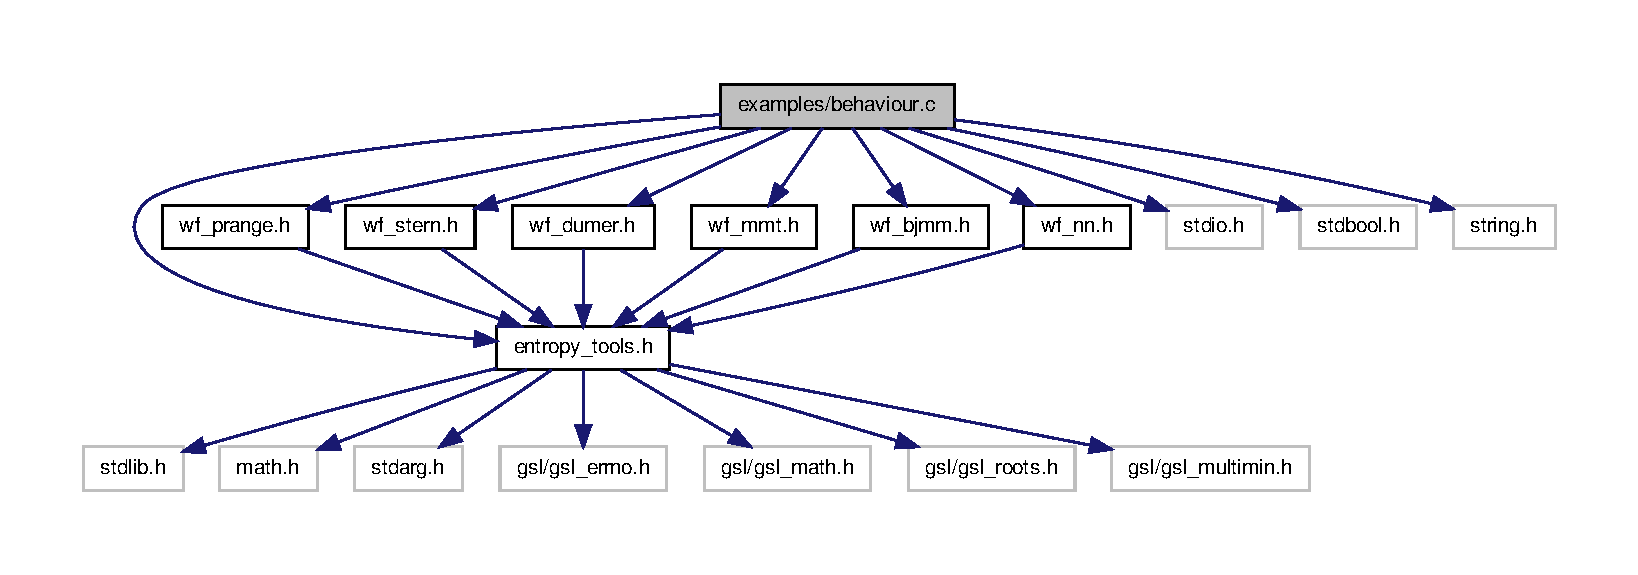
\includegraphics[width=350pt]{behaviour_8c__incl}
\end{center}
\end{figure}


\subsection*{\-Functions}
\begin{DoxyCompactItemize}
\item 
int \hyperlink{behaviour_8c_a0ddf1224851353fc92bfbff6f499fa97}{main} (int argc, char $\ast$argv\mbox{[}$\,$\mbox{]})

\item 
void \hyperlink{behaviour_8c_r0ddf1224851353fc92bfbff6f499fa97}{usage} ( void )
\end{DoxyCompactItemize}

\subsection*{\-Variables}
\begin{DoxyCompactItemize}
\item 
\-F\-I\-L\-E $\ast$ \hyperlink{behaviour_8c_aa3f2c1d3035c367b8891e613934cac98}{streamout}
\item 
\hyperlink{structwf__params}{wf\-\_\-params} \hyperlink{behaviour_8c_aea89d30d6c8cc9ac79ded86e7f78d3ad}{wfp}
\item 
double($\ast$ \hyperlink{behaviour_8c_a2254ed7d4ba79ef4b09f6801626aa1db}{wf\-\_\-algo} )(\hyperlink{structwf__params}{wf\-\_\-params} $\ast$)
\item 
char \hyperlink{behaviour_8c_ad7c92c302d8095e7b78a691e451ecf15}{algo} \mbox{[}20\mbox{]}
\end{DoxyCompactItemize}


\subsection{\-Detailed \-Description}
\-Example program, it shows wf/w vs w. \-For a code rate k, this program calculates wf/w respects the error rate w ( with values between 0 and \-Gilbert-\/\-Varshamov bound). \-We can see the wf/w becomes near to expect value -\/log\-\_\-2(1-\/k) when w approachs 0. 

\-Definition in file \hyperlink{behaviour_8c}{behaviour.\-c}.

\subsection{\-Function \-Documentation}
\hypertarget{behaviour_8c_a0ddf1224851353fc92bfbff6f499fa97}{\index{behaviour.\-c@{behaviour.\-c}!main@{main}}
\index{main@{main}!behaviour.c@{behaviour.\-c}}
\subsubsection[{main}]{\setlength{\rightskip}{0pt plus 5cm}int {\bf main} (
\begin{DoxyParamCaption}
\item[{int}]{argc, }
\item[{char $\ast$}]{argv\mbox{[}$\,$\mbox{]}}
\end{DoxyParamCaption}
)}}\label{behaviour_8c_a0ddf1224851353fc92bfbff6f499fa97}
\-It shows wf/w vs w. Definition at line 63 of file behaviour.\-c.


\hypertarget{behaviour_8c_r0ddf1224851353fc92bfbff6f499fa97}{\index{behaviour.\-c@{behaviour.\-c}!usage@{usage}}
\index{usage@{usage}!behaviour.c@{behaviour.\-c}}
\subsubsection[{usage}]{\setlength{\rightskip}{0pt plus 5cm}void {\bf usage} ( void )}}\label{behaviour_8c_r0ddf1224851353fc92bfbff6f499fa97}
\-It prints help. 

\-Definition at line 54 of file behaviour.\-c.


\subsection{\-Variable \-Documentation}
\hypertarget{behaviour_8c_ad7c92c302d8095e7b78a691e451ecf15}{\index{behaviour.\-c@{behaviour.\-c}!algo@{algo}}
\index{algo@{algo}!behaviour.c@{behaviour.\-c}}
\subsubsection[{algo}]{\setlength{\rightskip}{0pt plus 5cm}char {\bf algo}\mbox{[}20\mbox{]}}}\label{behaviour_8c_ad7c92c302d8095e7b78a691e451ecf15}

\-This variable contains the name of algorithm to use. 

\-Definition at line 46 of file behaviour.\-c.

\hypertarget{behaviour_8c_aa3f2c1d3035c367b8891e613934cac98}{\index{behaviour.\-c@{behaviour.\-c}!streamout@{streamout}}
\index{streamout@{streamout}!behaviour.c@{behaviour.\-c}}
\subsubsection[{streamout}]{\setlength{\rightskip}{0pt plus 5cm}\-F\-I\-L\-E$\ast$ {\bf streamout}}}\label{behaviour_8c_aa3f2c1d3035c367b8891e613934cac98}

\-This variable will saves in a file the obtained values after optimization of wf. 

\-Definition at line 43 of file behaviour.\-c.

\hypertarget{behaviour_8c_a2254ed7d4ba79ef4b09f6801626aa1db}{\index{behaviour.\-c@{behaviour.\-c}!wf\-\_\-algo@{wf\-\_\-algo}}
\index{wf\-\_\-algo@{wf\-\_\-algo}!behaviour.c@{behaviour.\-c}}
\subsubsection[{wf\-\_\-algo}]{\setlength{\rightskip}{0pt plus 5cm}double($\ast$  {\bf wf\-\_\-algo})({\bf wf\-\_\-params} $\ast$)}}\label{behaviour_8c_a2254ed7d4ba79ef4b09f6801626aa1db}


\-This variable saves the adress of the optimization function of work factor. 

\-Definition at line 45 of file behaviour.\-c.

\hypertarget{behaviour_8c_aea89d30d6c8cc9ac79ded86e7f78d3ad}{\index{behaviour.\-c@{behaviour.\-c}!wfp@{wfp}}
\index{wfp@{wfp}!behaviour.c@{behaviour.\-c}}
\subsubsection[{wfp}]{\setlength{\rightskip}{0pt plus 5cm}{\bf wf\-\_\-params} {\bf wfp}}}\label{behaviour_8c_aea89d30d6c8cc9ac79ded86e7f78d3ad}

\-This variable contains the value of k, w, wf/w, l, p, p1, p2 after optimization of wf. 

\-Definition at line 44 of file behaviour.\-c.


\hypertarget{bound_8c}{\section{examples/bound.c}
\label{bound_8c}\index{examples/bound.\-c@{examples/bound.\-c}}
}

\-Auxilairy program which calculates the index a of the bound fonction.  
\subsection*{Dependencies}

{\ttfamily \#include $<$entropy\-\_\-tools.\-h$>$}\*\\
{\ttfamily \#include $<$bound\-\_\-function.\-h$>$}\*\\
{\ttfamily \#include $<$wf\-\_\-prange.\-h$>$}\*\\
{\ttfamily \#include $<$wf\-\_\-stern.\-h$>$}\*\\
{\ttfamily \#include $<$wf\-\_\-dumer.\-h$>$}\*\\
{\ttfamily \#include $<$wf\-\_\-mmt.\-h$>$}\*\\
{\ttfamily \#include $<$wf\-\_\-bjmm.\-h$>$}\*\\
{\ttfamily \#include $<$wf\-\_\-nn.\-h$>$}\*\\
{\ttfamily \#include $<$stdio.\-h$>$}\*\\
{\ttfamily \#include $<$getopt.\-h$>$}\*\\

\-Include dependency graph for bound.\-c\-:
\nopagebreak
\begin{figure}[H]
\begin{center}
\leavevmode
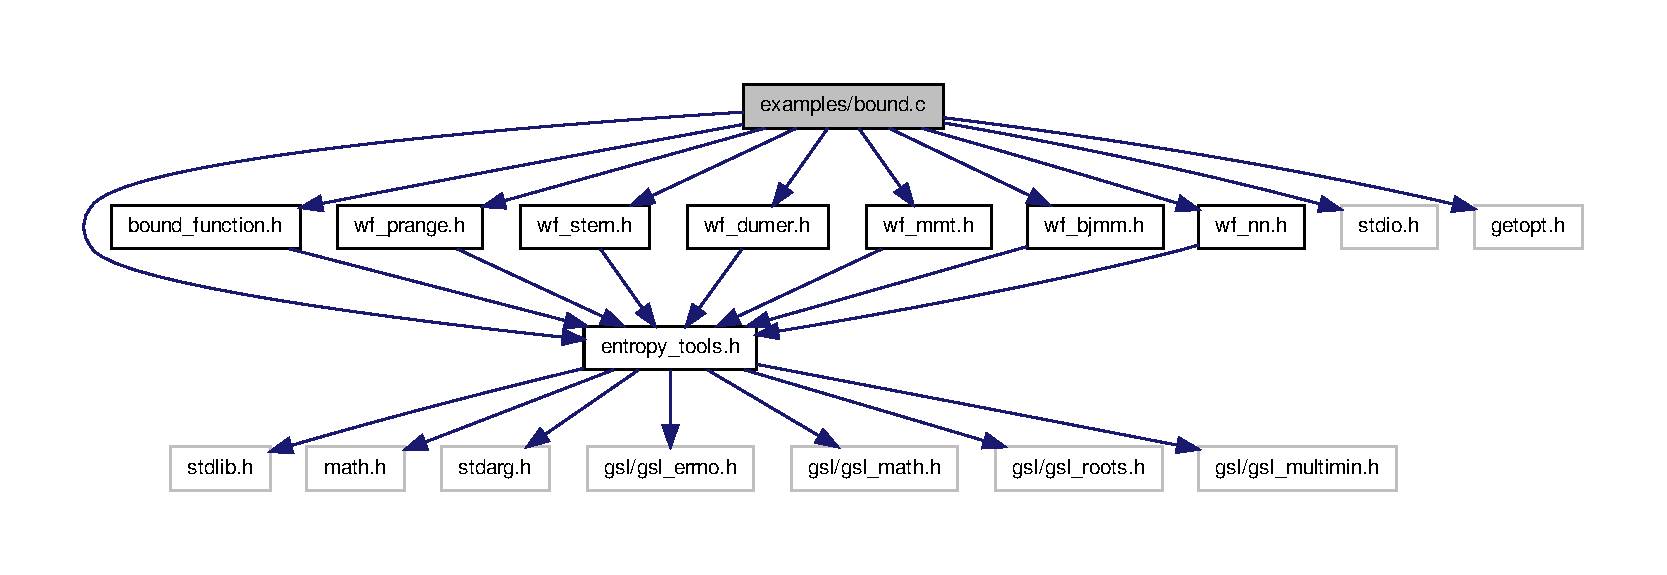
\includegraphics[width=350pt]{bound_8c__incl}
\end{center}
\end{figure}
\subsection*{\-Functions}
\begin{DoxyCompactItemize}
\item 
int \hyperlink{bound_8c_a0ddf1224851353fc92bfbff6f499fa97}{main} (int argc, char $\ast$argv\mbox{[}$\,$\mbox{]})

\item 
void  \hyperlink{bound_8c_r0ddf1224851353fc92bfbff6f499fa97}{usage} (void)
\end{DoxyCompactItemize}

\subsection*{\-Variables}
\begin{DoxyCompactItemize}
\item 
\-F\-I\-L\-E $\ast$ \hyperlink{bound_8c_aa3f2c1d3035c367b8891e613934cac98}{streamout}
\item 
\hyperlink{structwf__params}{wf\-\_\-params} \hyperlink{bound_8c_aea89d30d6c8cc9ac79ded86e7f78d3ad}{wfp}
\item 
double($\ast$ \hyperlink{bound_8c_a2254ed7d4ba79ef4b09f6801626aa1db}{wf\-\_\-algo} )(\hyperlink{structwf__params}{wf\-\_\-params} $\ast$)
\end{DoxyCompactItemize}


\subsection{\-Detailed \-Description}
\-Auxilairy program which calculates the index a of the bound fonction. \-This program takes a generic decoding algorithm algo as input and returns a in \mbox{]}0,1\mbox{[} such that min \-B\-\_\-a = \-W\-F(algo) for many code rate k in \mbox{[}0,1\mbox{]} ( and error rate w as \-Gilbert \-Varshamov's bound ). 

\-Definition in file \hyperlink{bound_8c}{bound.\-c}.

\subsection{\-Function \-Documentation}
\hypertarget{bound_8c_a0ddf1224851353fc92bfbff6f499fa97}{\index{bound.\-c@{bound.\-c}!main@{main}}
\index{main@{main}!bound.c@{bound.\-c}}
\subsubsection[{main}]{\setlength{\rightskip}{0pt plus 5cm}int {\bf main} (
\begin{DoxyParamCaption}
\item[{int}]{argc, }
\item[{char $\ast$}]{argv\mbox{[}$\,$\mbox{]}}
\end{DoxyParamCaption}
)}}\label{bound_8c_a0ddf1224851353fc92bfbff6f499fa97}

\-It calculates the index a of the bound fonction.

\-Definition at line 82 of file bound.\-c.

\hypertarget{bound_8c_r0ddf1224851353fc92bfbff6f499fa97}{\index{bound.\-c@{bound.\-c}!usage@{usage}}
\index{usage@{usage}!bound.c@{bound.\-c}}
\subsubsection[{usage}]{\setlength{\rightskip}{0pt plus 5cm}void {\bf usage} ( void )}}\label{bound_8c_r0ddf1224851353fc92bfbff6f499fa97}

It prints help.

\-Definition at line 54 of file bound.c.

\subsection{\-Variable \-Documentation}
\hypertarget{bound_8c_aa3f2c1d3035c367b8891e613934cac98}{\index{bound.\-c@{bound.\-c}!streamout@{streamout}}
\index{streamout@{streamout}!bound.c@{bound.\-c}}
\subsubsection[{streamout}]{\setlength{\rightskip}{0pt plus 5cm}\-F\-I\-L\-E$\ast$ {\bf streamout}}}\label{bound_8c_aa3f2c1d3035c367b8891e613934cac98}


\-This variable will saves in a file the obtained values after optimization of wf.

\-Definition at line 44 of file bound.\-c.

\hypertarget{bound_8c_a2254ed7d4ba79ef4b09f6801626aa1db}{\index{bound.\-c@{bound.\-c}!wf\-\_\-algo@{wf\-\_\-algo}}
\index{wf\-\_\-algo@{wf\-\_\-algo}!bound.c@{bound.\-c}}
\subsubsection[{wf\-\_\-algo}]{\setlength{\rightskip}{0pt plus 5cm}double($\ast$  {\bf wf\-\_\-algo})({\bf wf\-\_\-params} $\ast$)}}\label{bound_8c_a2254ed7d4ba79ef4b09f6801626aa1db}

\-This variable saves the adress of the optimization function of work factor.

\-Definition at line 45 of file bound.\-c.

\hypertarget{bound_8c_aea89d30d6c8cc9ac79ded86e7f78d3ad}{\index{bound.\-c@{bound.\-c}!wfp@{wfp}}
\index{wfp@{wfp}!bound.c@{bound.\-c}}
\subsubsection[{wfp}]{\setlength{\rightskip}{0pt plus 5cm}{\bf wf\-\_\-params} {\bf wfp}}}\label{bound_8c_aea89d30d6c8cc9ac79ded86e7f78d3ad}

\-This variable contains the value of k, w, wf/w, l, p, p1, p2 after optimization of wf.

\-Definition at line 46 of file bound.\-c.

\hypertarget{bound__function_8h}{\section{include/bound\-\_\-function.h \-File \-Reference}
\label{bound__function_8h}\index{include/bound\-\_\-function.\-h@{include/bound\-\_\-function.\-h}}
}
\-Library for calculation of \-Bound \-Function.  

\subsection*{Dependencies}
{\ttfamily \#include \char`\"{}entropy\-\_\-tools.\-h\char`\"{}}\*\\
{\ttfamily \#include $<$gsl/gsl\-\_\-roots.\-h$>$}\*\\

\-Include dependency graph for bound\-\_\-function.\-h\-:
\nopagebreak
\begin{figure}[H]
\begin{center}
\leavevmode
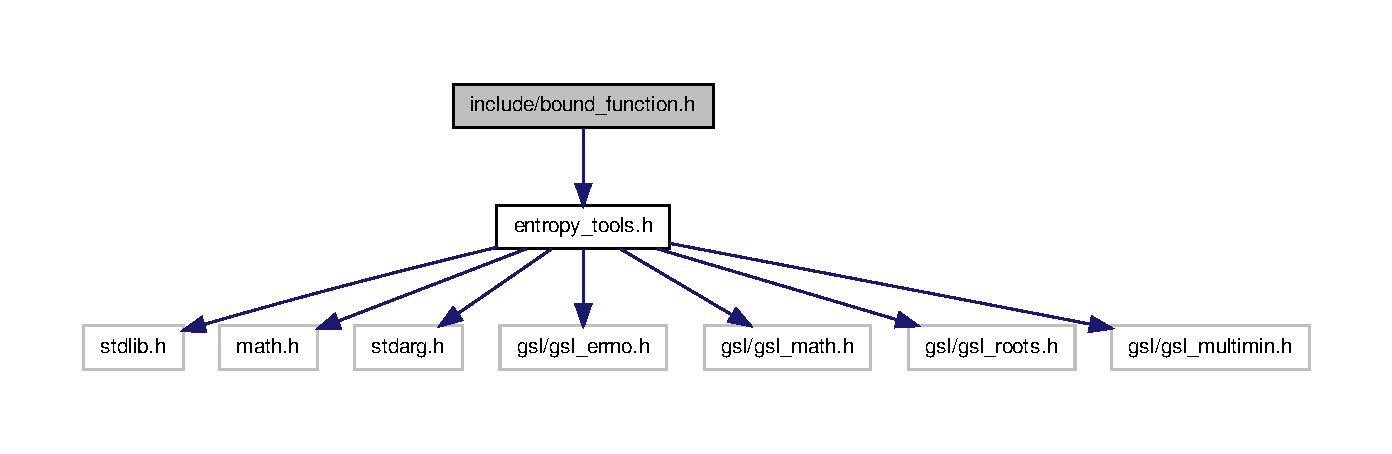
\includegraphics[width=350pt]{bound__function_8h__incl}
\end{center}
\end{figure}
\-This graph shows which files directly or indirectly include this file\-:
\nopagebreak
\begin{figure}[H]
\begin{center}
\leavevmode
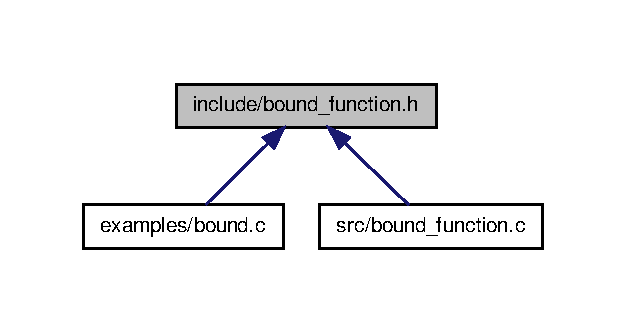
\includegraphics[width=300pt]{bound__function_8h__dep__incl}
\end{center}
\end{figure}

\subsection*{\-Defines}
\begin{DoxyCompactItemize}
\item 
\#define \hyperlink{bound__function_8h_a79a629c80cd09a3bbe52473b9c0c626a}{\-B\-O\-U\-N\-D\-\_\-\-F\-U\-N\-T\-I\-O\-N\-\_\-\-H}
\end{DoxyCompactItemize}
\subsection*{\-Functions}
\begin{DoxyCompactItemize}
\item 
double \hyperlink{bound__function_8h_a3861f0ee3f0966eaa504ae6e96a5538b}{pp} (double l, \hyperlink{structwf__params}{wf\-\_\-params} $\ast$params)
\item 
double \hyperlink{bound__function_8h_a4af35613987196849ea6b261a6d9939d}{dif\-\_\-pp} (double l, void $\ast$params)
\item 
double \hyperlink{bound__function_8h_a7e59befac1de8863e7bc694243fdc9c2}{pp\-\_\-df} (double l, \hyperlink{structwf__params}{wf\-\_\-params} $\ast$params)
\item 
double \hyperlink{bound__function_8h_a3af48831cb33dc02f5f72632592c8fc5}{reduced\-\_\-\-Ba} (double l, \hyperlink{structwf__params}{wf\-\_\-params} $\ast$params)
\item 
double \hyperlink{bound__function_8h_a18b7d91851ce5a2f94da2cb6ed20bc76}{reduced\-\_\-\-Ba\-\_\-df} (double l, void $\ast$params)
\item 
double \hyperlink{bound__function_8h_ae39e0703a1b025b97620c2fe2a17aed9}{l\-\_\-max} (\hyperlink{structwf__params}{wf\-\_\-params} $\ast$params)
\item 
double \hyperlink{bound__function_8h_a545abfeb71c0648db0a91dfa3e345e57}{\-Optimal\-\_\-reduced\-\_\-\-Ba} (\hyperlink{structwf__params}{wf\-\_\-params} $\ast$params)
\item 
double \hyperlink{bound__function_8h_ab965279f87e73cd3620cb491983ca3c4}{dif\-\_\-\-Optimal\-\_\-reduced\-\_\-\-Ba} (double a, void $\ast$params)
\item 
double \hyperlink{bound__function_8h_a806424a846d7c01ff8d78df2cf26c3ed}{find\-\_\-coefficient} (\hyperlink{structwf__params}{wf\-\_\-params} $\ast$params)
\end{DoxyCompactItemize}
\subsection{\-Detailed \-Description}
\-Library for calculation of \-Bound \-Function. \-This \-Library calculate theorical \-Bound \-Function, its optimal value for a coefficient a of min B\_a and find, for a work factor wf, the coefficient a for the equation min B\_a = wf for k, w fixed. 

\-Definition in file \hyperlink{bound__function_8h}{bound\-\_\-function.\-h}.



\subsection{\-Define \-Documentation}
\hypertarget{bound__function_8h_a79a629c80cd09a3bbe52473b9c0c626a}{\index{bound\-\_\-function.\-h@{bound\-\_\-function.\-h}!\-B\-O\-U\-N\-D\-\_\-\-F\-U\-N\-T\-I\-O\-N\-\_\-\-H@{\-B\-O\-U\-N\-D\-\_\-\-F\-U\-N\-T\-I\-O\-N\-\_\-\-H}}
\index{\-B\-O\-U\-N\-D\-\_\-\-F\-U\-N\-T\-I\-O\-N\-\_\-\-H@{\-B\-O\-U\-N\-D\-\_\-\-F\-U\-N\-T\-I\-O\-N\-\_\-\-H}!bound_function.h@{bound\-\_\-function.\-h}}
\subsubsection[{\-B\-O\-U\-N\-D\-\_\-\-F\-U\-N\-T\-I\-O\-N\-\_\-\-H}]{\setlength{\rightskip}{0pt plus 5cm}\#define {\bf \-B\-O\-U\-N\-D\-\_\-\-F\-U\-N\-T\-I\-O\-N\-\_\-\-H}}}\label{bound__function_8h_a79a629c80cd09a3bbe52473b9c0c626a}


\-Definition at line 31 of file bound\-\_\-function.\-h.



\subsection{\-Function \-Documentation}

\hypertarget{bound__function_8h_a3861f0ee3f0966eaa504ae6e96a5538b}{\index{bound\-\_\-function.\-h@{bound\-\_\-function.\-h}!pp@{pp}}
\index{pp@{pp}!bound_function.h@{bound\-\_\-function.\-h}}
\subsubsection[{pp}]{\setlength{\rightskip}{0pt plus 5cm}double {\bf pp} (
\begin{DoxyParamCaption}
\item[{double}]{l, }
\item[{{\bf wf\-\_\-params} $\ast$}]{params}
\end{DoxyParamCaption}
)}}\label{bound__function_8h_a3861f0ee3f0966eaa504ae6e96a5538b}


\-Calculates the p such that 2$^\wedge$l=binomial(k+l,ap). 

\-Declaration at line 42 of file bound\-\_\-function.\-h.

\hypertarget{bound__function_8h_a4af35613987196849ea6b261a6d9939d}{\index{bound\-\_\-function.\-h@{bound\-\_\-function.\-h}!dif\-\_\-pp@{dif\-\_\-pp}}
\index{dif\-\_\-pp@{dif\-\_\-pp}!bound_function.h@{bound\-\_\-function.\-h}}
\subsubsection[{dif\-\_\-pp}]{\setlength{\rightskip}{0pt plus 5cm}{\bf dif\-\_\-pp} (
\begin{DoxyParamCaption}
\item[{double}]{l, }
\item[{void $\ast$}]{params}
\end{DoxyParamCaption}
)}}\label{bound__function_8h_a4af35613987196849ea6b261a6d9939d}


the diference pp(l,a)-\/w. 

\-Declaration at line 49 of file bound\-\_\-function.\-h.

\hypertarget{bound__function_8h_a7e59befac1de8863e7bc694243fdc9c2}{\index{bound\-\_\-function.\-h@{bound\-\_\-function.\-h}!pp\-\_\-df@{pp\-\_\-df}}
\index{pp\-\_\-df@{pp\-\_\-df}!bound_function.h@{bound\-\_\-function.\-h}}
\subsubsection[{pp\-\_\-df}]{\setlength{\rightskip}{0pt plus 5cm}{\bf pp\-\_\-df} (
\begin{DoxyParamCaption}
\item[{double}]{l, }
\item[{{\bf wf\-\_\-params} $\ast$}]{params}
\end{DoxyParamCaption}
)}}\label{bound__function_8h_a7e59befac1de8863e7bc694243fdc9c2}


\-Derivate of function pp. 

\-Declaration at line 56 of file bound\-\_\-function.\-h.

\hypertarget{bound__function_8h_a3af48831cb33dc02f5f72632592c8fc5}{\index{bound\-\_\-function.\-h@{bound\-\_\-function.\-h}!reduced\-\_\-\-Ba@{reduced\-\_\-\-Ba}}
\index{reduced\-\_\-\-Ba@{reduced\-\_\-\-Ba}!bound_function.h@{bound\-\_\-function.\-h}}
\subsubsection[{reduced\-\_\-\-Ba}]{\setlength{\rightskip}{0pt plus 5cm}double {\bf reduced\-\_\-\-Ba} (
\begin{DoxyParamCaption}
\item[{double}]{l, }
\item[{{\bf wf\-\_\-params} $\ast$}]{params}
\end{DoxyParamCaption}
)}}\label{bound__function_8h_a3af48831cb33dc02f5f72632592c8fc5}


\-Reduced version of \-Ba(l,p). This function will achieve the same minimum value of function \-Ba(l,p). 

\-Declaration at line 65 of file bound\-\_\-function.\-h.


\hypertarget{bound__function_8h_a18b7d91851ce5a2f94da2cb6ed20bc76}{\index{bound\-\_\-function.\-h@{bound\-\_\-function.\-h}!reduced\-\_\-\-Ba\-\_\-df@{reduced\-\_\-\-Ba\-\_\-df}}
\index{reduced\-\_\-\-Ba\-\_\-df@{reduced\-\_\-\-Ba\-\_\-df}!bound_function.h@{bound\-\_\-function.\-h}}
\subsubsection[{reduced\-\_\-\-Ba\-\_\-df}]{\setlength{\rightskip}{0pt plus 5cm}double {\bf reduced\-\_\-\-Ba\-\_\-df} (
\begin{DoxyParamCaption}
\item[{double}]{l, }
\item[{void $\ast$}]{params}
\end{DoxyParamCaption}
)}}\label{bound__function_8h_a18b7d91851ce5a2f94da2cb6ed20bc76}


\-Derivate of function reduced\-\_\-\-Ba. 

\-Declaration at line 72 of file bound\-\_\-function.\-h.

\hypertarget{bound__function_8h_ae39e0703a1b025b97620c2fe2a17aed9}{\index{bound\-\_\-function.\-h@{bound\-\_\-function.\-h}!l\-\_\-max@{l\-\_\-max}}
\index{l\-\_\-max@{l\-\_\-max}!bound_function.h@{bound\-\_\-function.\-h}}
\subsubsection[{l\-\_\-max}]{\setlength{\rightskip}{0pt plus 5cm}double {\bf l\-\_\-max} (
\begin{DoxyParamCaption}
\item[{{\bf wf\-\_\-params} $\ast$}]{params}
\end{DoxyParamCaption}
)}}\label{bound__function_8h_ae39e0703a1b025b97620c2fe2a17aed9}


\-Obtains the maximum value of l such \-Ba is calculable. 

\-Declaration at line 79 of file bound\-\_\-function.\-h.


\hypertarget{bound__function_8h_a545abfeb71c0648db0a91dfa3e345e57}{\index{bound\-\_\-function.\-h@{bound\-\_\-function.\-h}!\-Optimal\-\_\-reduced\-\_\-\-Ba@{\-Optimal\-\_\-reduced\-\_\-\-Ba}}
\index{\-Optimal\-\_\-reduced\-\_\-\-Ba@{\-Optimal\-\_\-reduced\-\_\-\-Ba}!bound_function.h@{bound\-\_\-function.\-h}}
\subsubsection[{\-Optimal\-\_\-reduced\-\_\-\-Ba}]{\setlength{\rightskip}{0pt plus 5cm}double {\bf \-Optimal\-\_\-reduced\-\_\-\-Ba} (
\begin{DoxyParamCaption}
\item[{{\bf wf\-\_\-params} $\ast$}]{params}
\end{DoxyParamCaption}
)}}\label{bound__function_8h_a545abfeb71c0648db0a91dfa3e345e57}


\-Obtains the minimum value of \-Ba. 

\-Declaration at line 86 of file bound\-\_\-function.\-h.



\hypertarget{bound__function_8h_ab965279f87e73cd3620cb491983ca3c4}{\index{bound\-\_\-function.\-h@{bound\-\_\-function.\-h}!dif\-\_\-\-Optimal\-\_\-reduced\-\_\-\-Ba@{dif\-\_\-\-Optimal\-\_\-reduced\-\_\-\-Ba}}
\index{dif\-\_\-\-Optimal\-\_\-reduced\-\_\-\-Ba@{dif\-\_\-\-Optimal\-\_\-reduced\-\_\-\-Ba}!bound_function.h@{bound\-\_\-function.\-h}}
\subsubsection[{dif\-\_\-\-Optimal\-\_\-reduced\-\_\-\-Ba}]{\setlength{\rightskip}{0pt plus 5cm}double {\bf dif\-\_\-\-Optimal\-\_\-reduced\-\_\-\-Ba} (
\begin{DoxyParamCaption}
\item[{double}]{a, }
\item[{void $\ast$}]{params}
\end{DoxyParamCaption}
)}}\label{bound__function_8h_ab965279f87e73cd3620cb491983ca3c4}


\-The difference \-Optimal\-\_\-reduced\-\_\-\-Ba -\/ workfactor. 

\-Declaration at line 93 of file bound\-\_\-function.\-h.



\hypertarget{bound__function_8h_a806424a846d7c01ff8d78df2cf26c3ed}{\index{bound\-\_\-function.\-h@{bound\-\_\-function.\-h}!find\-\_\-coefficient@{find\-\_\-coefficient}}
\index{find\-\_\-coefficient@{find\-\_\-coefficient}!bound_function.h@{bound\-\_\-function.\-h}}
\subsubsection[{find\-\_\-coefficient}]{\setlength{\rightskip}{0pt plus 5cm}double {\bf find\-\_\-coefficient} (
\begin{DoxyParamCaption}
\item[{{\bf wf\-\_\-params} $\ast$}]{params}
\end{DoxyParamCaption}
)}}\label{bound__function_8h_a806424a846d7c01ff8d78df2cf26c3ed}


\-Find a such that reduced\-\_\-\-Ba\-\_\-min(a)=wf. 

\-Declaration at line 100 of file bound\-\_\-function.\-h.





\hypertarget{entropy__tools_8h}{\section{include/entropy\-\_\-tools.h \-File \-Reference}
\label{entropy__tools_8h}\index{include/entropy\-\_\-tools.\-h@{include/entropy\-\_\-tools.\-h}}
}


\-Auxiliary library for calculation of \-Work \-Factor.  

\subsection*{Dependencies}
{\ttfamily \#include $<$stdlib.\-h$>$}\*\\
{\ttfamily \#include $<$math.\-h$>$}\*\\
{\ttfamily \#include $<$stdarg.\-h$>$}\*\\
{\ttfamily \#include $<$gsl/gsl\-\_\-errno.\-h$>$}\*\\
{\ttfamily \#include $<$gsl/gsl\-\_\-math.\-h$>$}\*\\
{\ttfamily \#include $<$gsl/gsl\-\_\-roots.\-h$>$}\*\\
{\ttfamily \#include $<$gsl/gsl\-\_\-multimin.\-h$>$}\*\\

\-Include dependency graph for entropy\-\_\-tools.\-h\-:
\nopagebreak
\begin{figure}[H]
\begin{center}
\leavevmode
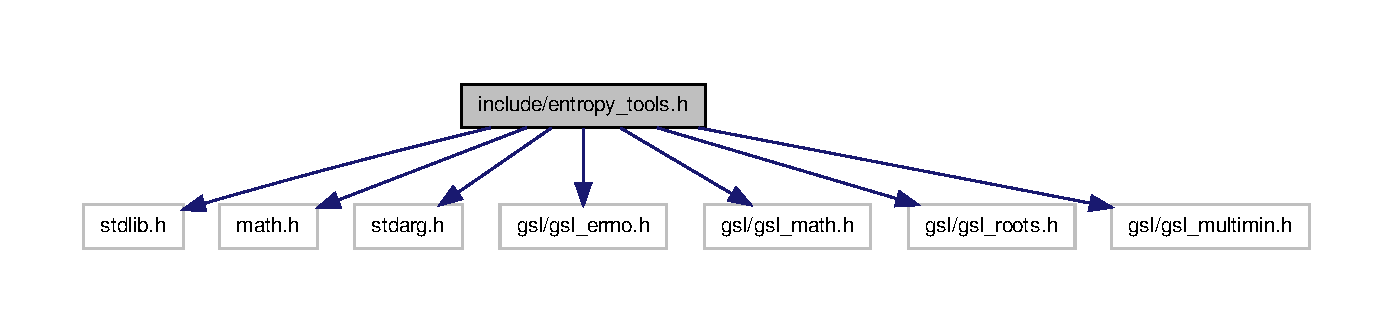
\includegraphics[width=350pt]{entropy__tools_8h__incl}
\end{center}
\end{figure}
\-This graph shows which files directly or indirectly include this file\-:
\nopagebreak
\begin{figure}[H]
\begin{center}
\leavevmode
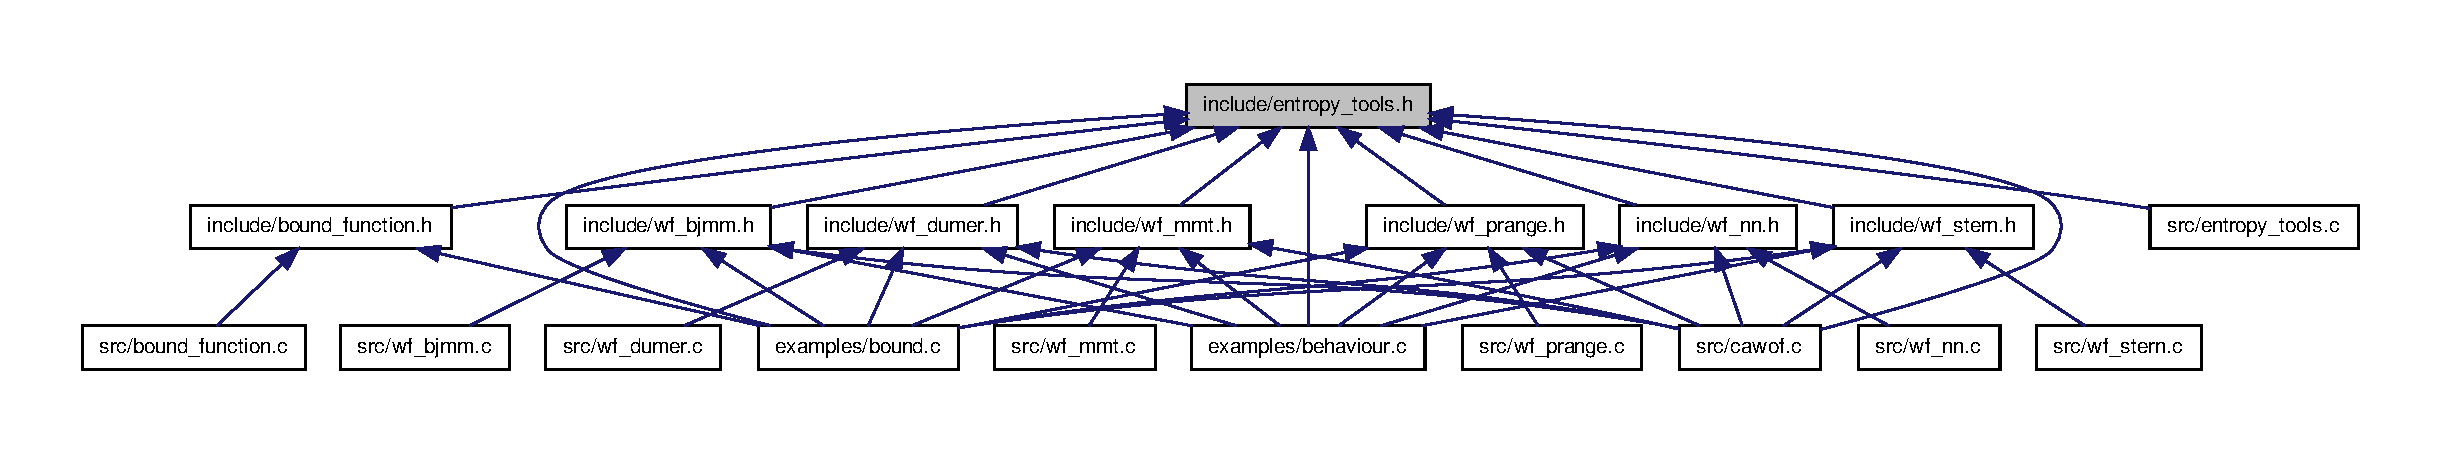
\includegraphics[width=350pt]{entropy__tools_8h__dep__incl}
\end{center}
\end{figure}


\subsection*{\-Data \-Structures}
\begin{DoxyCompactItemize}
\item 
struct \hyperlink{structwf__params}{wf\-\_\-params}
\end{DoxyCompactItemize}
\subsection*{\-Functions}
\begin{DoxyCompactItemize}
\item 
double \hyperlink{entropy__tools_8h_ac4be1977864445c9d3676c1caf020435}{min} (double x, double y)
\item 
double \hyperlink{entropy__tools_8h_aceeb951e1b17504f8d543719bd202818}{max} (int num,...)
\item 
double \hyperlink{entropy__tools_8h_a990759dbbe88d82fc69c6800d5951e94}{entropy} (double x)
\item 
double \hyperlink{entropy__tools_8h_a6177deb9e0879434f5faf04e0bacbc60}{dif\-\_\-entropy} (double x, void $\ast$params)
\item 
double \hyperlink{entropy__tools_8h_a982f069270a89ba48bcf6f1094664de9}{binomial} (double x, double y)
\item 
double \hyperlink{entropy__tools_8h_a58658edd80dde5f9f1f3dfb0ef5c3ad0}{entropy\-\_\-df} (double x, void $\ast$params)
\item 
void \hyperlink{entropy__tools_8h_a97ccbb83b56c2e90f48e07e6a97dabb0}{entropy\-\_\-fdf} (double x, void $\ast$params, double $\ast$y, double $\ast$dy)
\item 
double \hyperlink{entropy__tools_8h_afbd7396514b366c122f2021ca8820bce}{entropy\-\_\-inverse} (double y)
\end{DoxyCompactItemize}


\subsection{\-Detailed \-Description}
\-Auxiliary library for calculation of \-Work \-Factor. \-This \-Library contains the structure \hyperlink{structwf__params}{wf\-\_\-params} which comunicate several parameters in the optimization of several work factors. 

\-Definition in file \hyperlink{entropy__tools_8h}{entropy\-\_\-tools.\-h}.



\subsection{\-Function \-Documentation}

\hypertarget{entropy__tools_8h_ac4be1977864445c9d3676c1caf020435}{\index{entropy\-\_\-tools.\-h@{entropy\-\_\-tools.\-h}!min@{min}}
\index{min@{min}!entropy_tools.h@{entropy\-\_\-tools.\-h}}
\subsubsection[{min}]{\setlength{\rightskip}{0pt plus 5cm}{\bf min} (
\begin{DoxyParamCaption}
\item[{double}]{x, }
\item[{double}]{y}
\end{DoxyParamCaption}
)}}\label{entropy__tools_8h_ac4be1977864445c9d3676c1caf020435}


\-Minimum of two double values. 

\-Declaration at line 58 of file entropy\-\_\-tools.\-h.

\hypertarget{entropy__tools_8h_aceeb951e1b17504f8d543719bd202818}{\index{entropy\-\_\-tools.\-h@{entropy\-\_\-tools.\-h}!max@{max}}
\index{max@{max}!entropy_tools.h@{entropy\-\_\-tools.\-h}}
\subsubsection[{max}]{\setlength{\rightskip}{0pt plus 5cm}{\bf max} (
\begin{DoxyParamCaption}
\item[{int}]{num, }
\item[{}]{...}
\end{DoxyParamCaption}
)}}\label{entropy__tools_8h_aceeb951e1b17504f8d543719bd202818}


\-Maximum of num double values. 

\-Declaration at line 65 of file entropy\-\_\-tools.\-h.

\hypertarget{entropy__tools_8h_a990759dbbe88d82fc69c6800d5951e94}{\index{entropy\-\_\-tools.\-h@{entropy\-\_\-tools.\-h}!entropy@{entropy}}
\index{entropy@{entropy}!entropy_tools.h@{entropy\-\_\-tools.\-h}}
\subsubsection[{entropy}]{\setlength{\rightskip}{0pt plus 5cm}{\bf entropy} (
\begin{DoxyParamCaption}
\item[{double}]{x}
\end{DoxyParamCaption}
)}}\label{entropy__tools_8h_a990759dbbe88d82fc69c6800d5951e94}


\-This function calculates the (binary) entropy. 

\-Declaration at line 72 of file entropy\-\_\-tools.\-h.

\hypertarget{entropy__tools_8h_a6177deb9e0879434f5faf04e0bacbc60}{\index{entropy\-\_\-tools.\-h@{entropy\-\_\-tools.\-h}!dif\-\_\-entropy@{dif\-\_\-entropy}}
\index{dif\-\_\-entropy@{dif\-\_\-entropy}!entropy_tools.h@{entropy\-\_\-tools.\-h}}
\subsubsection[{dif\-\_\-entropy}]{\setlength{\rightskip}{0pt plus 5cm}{\bf dif\-\_\-entropy} (
\begin{DoxyParamCaption}
\item[{double}]{x, }
\item[{void $\ast$}]{params}
\end{DoxyParamCaption}
)}}\label{entropy__tools_8h_a6177deb9e0879434f5faf04e0bacbc60}

\-The diference entropy(x)-\/params. 

\-Declaration at line 79 of file entropy\-\_\-tools.\-h.

\hypertarget{entropy__tools_8h_a982f069270a89ba48bcf6f1094664de9}{\index{entropy\-\_\-tools.\-h@{entropy\-\_\-tools.\-h}!binomial@{binomial}}
\index{binomial@{binomial}!entropy_tools.h@{entropy\-\_\-tools.\-h}}
\subsubsection[{binomial}]{\setlength{\rightskip}{0pt plus 5cm}{\bf binomial} (
\begin{DoxyParamCaption}
\item[{double}]{x, }
\item[{double}]{y}
\end{DoxyParamCaption}
)}}\label{entropy__tools_8h_a982f069270a89ba48bcf6f1094664de9}

\-This function approximates \-Binomial coefficient by entropy function. 

\-Declaration at line 86 of file entropy\-\_\-tools.\-h.


\hypertarget{entropy__tools_8h_a58658edd80dde5f9f1f3dfb0ef5c3ad0}{\index{entropy\-\_\-tools.\-h@{entropy\-\_\-tools.\-h}!entropy\-\_\-df@{entropy\-\_\-df}}
\index{entropy\-\_\-df@{entropy\-\_\-df}!entropy_tools.h@{entropy\-\_\-tools.\-h}}
\subsubsection[{entropy\-\_\-df}]{\setlength{\rightskip}{0pt plus 5cm}{\bf entropy\-\_\-df} (
\begin{DoxyParamCaption}
\item[{double}]{x, }
\item[{void $\ast$}]{params}
\end{DoxyParamCaption}
)}}\label{entropy__tools_8h_a58658edd80dde5f9f1f3dfb0ef5c3ad0}


\-Derivate of entropy function. 

\-Declaration at line 93 of file entropy\-\_\-tools.\-h.

\hypertarget{entropy__tools_8h_a97ccbb83b56c2e90f48e07e6a97dabb0}{\index{entropy\-\_\-tools.\-h@{entropy\-\_\-tools.\-h}!entropy\-\_\-fdf@{entropy\-\_\-fdf}}
\index{entropy\-\_\-fdf@{entropy\-\_\-fdf}!entropy_tools.h@{entropy\-\_\-tools.\-h}}
\subsubsection[{entropy\-\_\-fdf}]{\setlength{\rightskip}{0pt plus 5cm}{\bf entropy\-\_\-fdf} (
\begin{DoxyParamCaption}
\item[{double}]{x, }
\item[{void $\ast$}]{params, }
\item[{double $\ast$}]{y, }
\item[{double $\ast$}]{dy}
\end{DoxyParamCaption}
)}}\label{entropy__tools_8h_a97ccbb83b56c2e90f48e07e6a97dabb0}

\-Obtains the dif\-\_\-entropy function and its derivate. 

\-Declaration at line 100 of file entropy\-\_\-tools.\-h.

\hypertarget{entropy__tools_8h_afbd7396514b366c122f2021ca8820bce}{\index{entropy\-\_\-tools.\-h@{entropy\-\_\-tools.\-h}!entropy\-\_\-inverse@{entropy\-\_\-inverse}}
\index{entropy\-\_\-inverse@{entropy\-\_\-inverse}!entropy_tools.h@{entropy\-\_\-tools.\-h}}
\subsubsection[{entropy\-\_\-inverse}]{\setlength{\rightskip}{0pt plus 5cm}{\bf entropy\-\_\-inverse} (
\begin{DoxyParamCaption}
\item[{double}]{y}
\end{DoxyParamCaption}
)}}\label{entropy__tools_8h_afbd7396514b366c122f2021ca8820bce}


\-Obtains the inverse of entropy function and return a real in \mbox{[}0,0.\-5\mbox{]}. 

\-Declaration at line 107 of file entropy\-\_\-tools.\-h.
\hypertarget{wf__bjmm_8h}{\section{include/wf\-\_\-bjmm.h \-File \-Reference}
\label{wf__bjmm_8h}\index{include/wf\-\_\-bjmm.\-h@{include/wf\-\_\-bjmm.\-h}}
}


\-Library for calculation of \-B\-J\-M\-M's \-Work \-Factor.  

\subsection*{Dependencies}

{\ttfamily \#include \char`\"{}entropy\-\_\-tools.\-h\char`\"{}}\*\\

\-Include dependency graph for wf\-\_\-bjmm.\-h\-:
\nopagebreak
\begin{figure}[H]
\begin{center}
\leavevmode
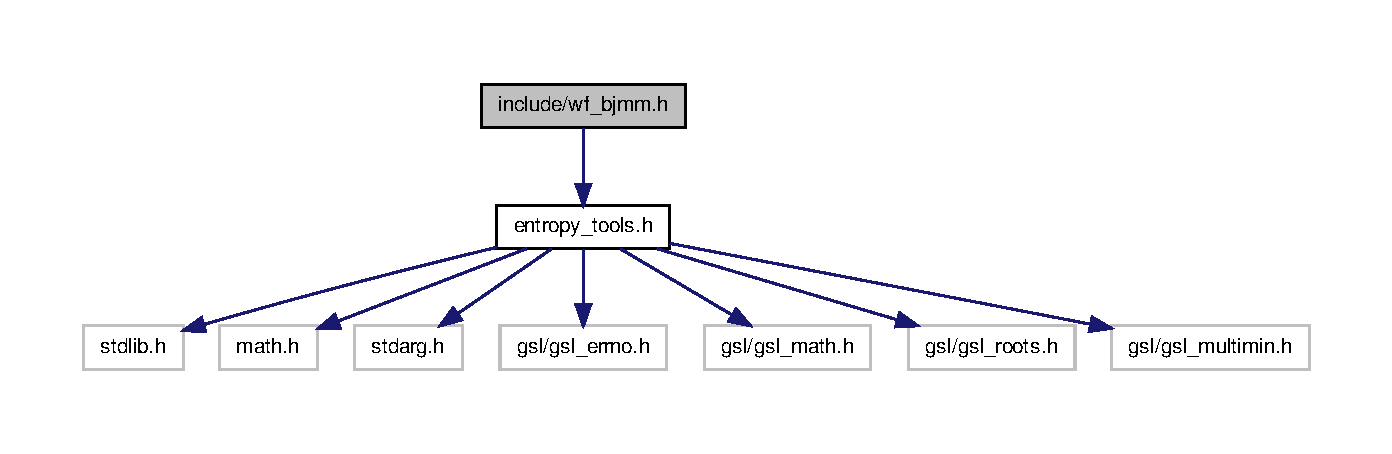
\includegraphics[width=350pt]{wf__bjmm_8h__incl}
\end{center}
\end{figure}
\-This graph shows which files directly or indirectly include this file\-:
\nopagebreak
\begin{figure}[H]
\begin{center}
\leavevmode
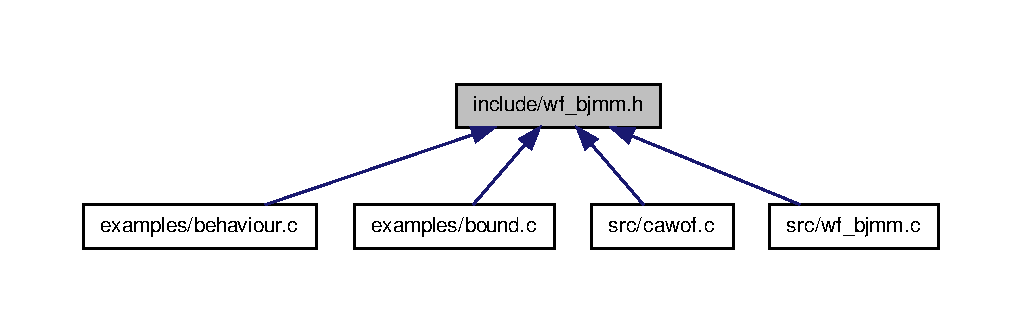
\includegraphics[width=350pt]{wf__bjmm_8h__dep__incl}
\end{center}
\end{figure}



\subsection*{\-Functions}
\begin{DoxyCompactItemize}
\item 
double \hyperlink{wf__bjmm_8h_afb4fca4c10e792952c64c8d712f44947}{wf\-\_\-\-B\-J\-M\-M} (const gsl\-\_\-vector $\ast$v, void $\ast$paramslp)
\item 
double \hyperlink{wf__bjmm_8h_a57582cc5476f2d16374afc1052b5a492}{\-Optimal\-\_\-wf\-\_\-\-B\-J\-M\-M\-\_\-p12} (const gsl\-\_\-vector $\ast$vv, void $\ast$params)
\item 
double \hyperlink{wf__bjmm_8h_aa1a2efb0ac81db558018172e12d0958d}{\-Optimal\-\_\-wf\-\_\-\-B\-J\-M\-M} (\hyperlink{structwf__params}{wf\-\_\-params} $\ast$params)
\end{DoxyCompactItemize}


\subsection{\-Detailed \-Description}
\-Library for calculation of \-B\-J\-M\-M's \-Work \-Factor. 

\-Definition in file \hyperlink{wf__bjmm_8h}{wf\-\_\-bjmm.\-h}.



\subsection{\-Function \-Documentation}

\hypertarget{wf__bjmm_8h_afb4fca4c10e792952c64c8d712f44947}{\index{wf\-\_\-bjmm.\-h@{wf\-\_\-bjmm.\-h}!wf\-\_\-\-B\-J\-M\-M@{wf\-\_\-\-B\-J\-M\-M}}
\index{wf\-\_\-\-B\-J\-M\-M@{wf\-\_\-\-B\-J\-M\-M}!wf_bjmm.h@{wf\-\_\-bjmm.\-h}}
\subsubsection[{wf\-\_\-\-B\-J\-M\-M}]{\setlength{\rightskip}{0pt plus 5cm}double {\bf wf\-\_\-\-B\-J\-M\-M} (
\begin{DoxyParamCaption}
\item[{const gsl\-\_\-vector $\ast$}]{v, }
\item[{void $\ast$}]{paramslp}
\end{DoxyParamCaption}
)}}\label{wf__bjmm_8h_afb4fca4c10e792952c64c8d712f44947}


Work Factor of BJMM's algorithm. Parameters p1 and p2 in v and k, w, N, l ,p in paramslp. 

\-Declaration at line 37 of file wf\-\_\-bjmm.\-h.

\hypertarget{wf__bjmm_8h_a57582cc5476f2d16374afc1052b5a492}{\index{wf\-\_\-bjmm.\-h@{wf\-\_\-bjmm.\-h}!\-Optimal\-\_\-wf\-\_\-\-B\-J\-M\-M\-\_\-p12@{\-Optimal\-\_\-wf\-\_\-\-B\-J\-M\-M\-\_\-p12}}
\index{\-Optimal\-\_\-wf\-\_\-\-B\-J\-M\-M\-\_\-p12@{\-Optimal\-\_\-wf\-\_\-\-B\-J\-M\-M\-\_\-p12}!wf_bjmm.h@{wf\-\_\-bjmm.\-h}}
\subsubsection[{\-Optimal\-\_\-wf\-\_\-\-B\-J\-M\-M\-\_\-p12}]{\setlength{\rightskip}{0pt plus 5cm}double {\bf \-Optimal\-\_\-wf\-\_\-\-B\-J\-M\-M\-\_\-p12} (
\begin{DoxyParamCaption}
\item[{const gsl\-\_\-vector $\ast$}]{vv, }
\item[{void $\ast$}]{params}
\end{DoxyParamCaption}
)}}\label{wf__bjmm_8h_a57582cc5476f2d16374afc1052b5a492}

\-Optimal \-Work \-Factor of \-B\-J\-M\-M's algorithm for l and p fixed. Parameters l and p in vv and k, w, \-N in params. It saves \-Optimal \-Parameters p1 and p2 in paramslp. 
 
 
 \-Declaration at line 47 of file wf\-\_\-bjmm.\-h.

\hypertarget{wf__bjmm_8h_aa1a2efb0ac81db558018172e12d0958d}{\index{wf\-\_\-bjmm.\-h@{wf\-\_\-bjmm.\-h}!\-Optimal\-\_\-wf\-\_\-\-B\-J\-M\-M@{\-Optimal\-\_\-wf\-\_\-\-B\-J\-M\-M}}
\index{\-Optimal\-\_\-wf\-\_\-\-B\-J\-M\-M@{\-Optimal\-\_\-wf\-\_\-\-B\-J\-M\-M}!wf_bjmm.h@{wf\-\_\-bjmm.\-h}}
\subsubsection[{\-Optimal\-\_\-wf\-\_\-\-B\-J\-M\-M}]{\setlength{\rightskip}{0pt plus 5cm}double {\bf \-Optimal\-\_\-wf\-\_\-\-B\-J\-M\-M} (
\begin{DoxyParamCaption}
\item[{{\bf wf\-\_\-params} $\ast$}]{params}
\end{DoxyParamCaption}
)}}\label{wf__bjmm_8h_aa1a2efb0ac81db558018172e12d0958d}

\-Optimal \-Work \-Factor of \-B\-J\-M\-M's algorithm. Parameters k, w, \-N in params. \-It saves \-Optimal \-Parameters l, p, p1 and p2 in params. 


\-Declaration at line 57 of file wf\-\_\-bjmm.\-h.



\hypertarget{wf__dumer_8h}{\section{include/wf\-\_\-dumer.h \-File \-Reference}
\label{wf__dumer_8h}\index{include/wf\-\_\-dumer.\-h@{include/wf\-\_\-dumer.\-h}}
}

\-Library for calculation of \-Dumer's \-Work \-Factor.  

\subsection*{Dependencies}
{\ttfamily \#include \char`\"{}entropy\-\_\-tools.\-h\char`\"{}}\*\\

\-Include dependency graph for wf\-\_\-dumer.\-h\-:
\nopagebreak
\begin{figure}[H]
\begin{center}
\leavevmode
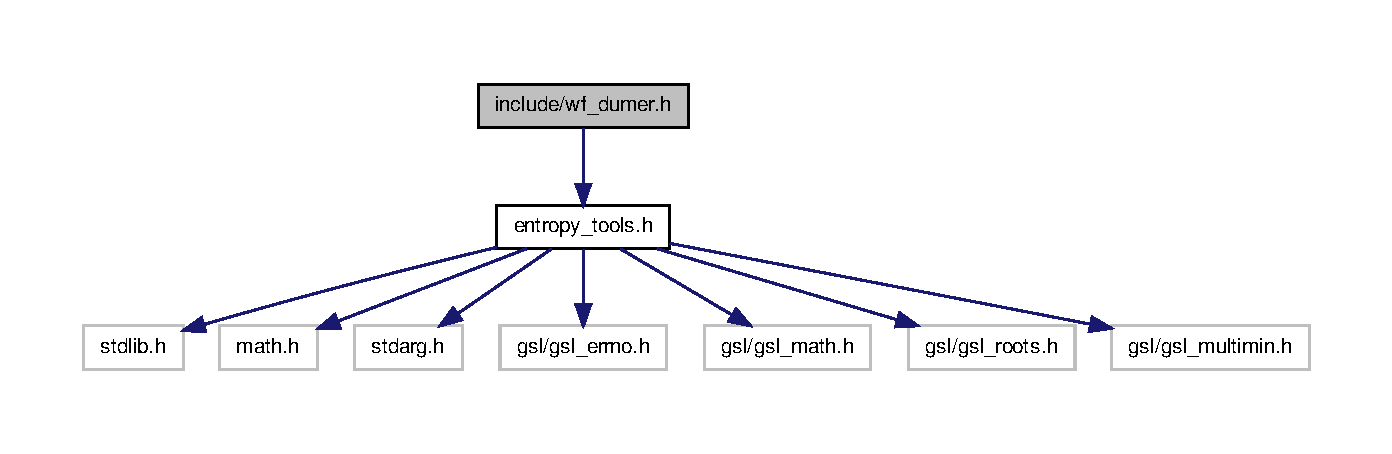
\includegraphics[width=350pt]{wf__dumer_8h__incl}
\end{center}
\end{figure}
\-This graph shows which files directly or indirectly include this file\-:
\nopagebreak
\begin{figure}[H]
\begin{center}
\leavevmode
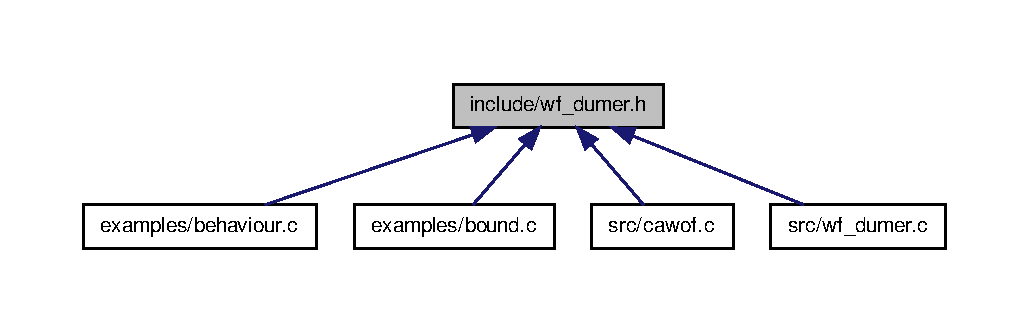
\includegraphics[width=350pt]{wf__dumer_8h__dep__incl}
\end{center}
\end{figure}



\subsection*{\-Functions}
\begin{DoxyCompactItemize}
\item 
double \hyperlink{wf__dumer_8h_a5244b19be3abd3f78ed6cca7ecd7a01e}{wf\-\_\-\-Dumer} (const gsl\-\_\-vector $\ast$v, void $\ast$params)
\item 
double \hyperlink{wf__dumer_8h_a479daa36a2e80f4a1432e4d4b027f8a3}{\-Optimal\-\_\-wf\-\_\-\-Dumer} (\hyperlink{structwf__params}{wf\-\_\-params} $\ast$params)
\end{DoxyCompactItemize}


\subsection{\-Detailed \-Description}
\-Library for calculation of \-Dumer's \-Work \-Factor. 

\-Definition in file \hyperlink{wf__dumer_8h}{wf\-\_\-dumer.\-h}.

\subsection{\-Function \-Documentation}

\hypertarget{wf__dumer_8h_a5244b19be3abd3f78ed6cca7ecd7a01e}{\index{wf\-\_\-dumer.\-h@{wf\-\_\-dumer.\-h}!wf\-\_\-\-Dumer@{wf\-\_\-\-Dumer}}
\index{wf\-\_\-\-Dumer@{wf\-\_\-\-Dumer}!wf_dumer.h@{wf\-\_\-dumer.\-h}}
\subsubsection[{wf\-\_\-\-Dumer}]{\setlength{\rightskip}{0pt plus 5cm}double {\bf wf\-\_\-\-Dumer} (
\begin{DoxyParamCaption}
\item[{const gsl\-\_\-vector $\ast$}]{v, }
\item[{void $\ast$}]{params}
\end{DoxyParamCaption}
)}}\label{wf__dumer_8h_a5244b19be3abd3f78ed6cca7ecd7a01e}

Work Factor of Dumer's algorithm. Parameters l and p in v and k, w, N in params. 

\-Definition at line 37 of file wf\-\_\-dumer.\-h.

\hypertarget{wf__dumer_8h_a479daa36a2e80f4a1432e4d4b027f8a3}{\index{wf\-\_\-dumer.\-h@{wf\-\_\-dumer.\-h}!\-Optimal\-\_\-wf\-\_\-\-Dumer@{\-Optimal\-\_\-wf\-\_\-\-Dumer}}
\index{\-Optimal\-\_\-wf\-\_\-\-Dumer@{\-Optimal\-\_\-wf\-\_\-\-Dumer}!wf_dumer.h@{wf\-\_\-dumer.\-h}}
\subsubsection[{\-Optimal\-\_\-wf\-\_\-\-Dumer}]{\setlength{\rightskip}{0pt plus 5cm}double {\bf \-Optimal\-\_\-wf\-\_\-\-Dumer} (
\begin{DoxyParamCaption}
\item[{{\bf wf\-\_\-params} $\ast$}]{params}
\end{DoxyParamCaption}
)}}\label{wf__dumer_8h_a479daa36a2e80f4a1432e4d4b027f8a3}

Optimal Work Factor of Dumer's algorithm. Parameters k, w, N in params. It saves Optimal Parameters l and p in params. 

\-Definition at line 46 of file wf\-\_\-dumer.\-h.



\hypertarget{wf__mmt_8h}{\section{include/wf\-\_\-mmt.h \-File \-Reference}
\label{wf__mmt_8h}\index{include/wf\-\_\-mmt.\-h@{include/wf\-\_\-mmt.\-h}}
}


\-Library for calculation of \-M\-M\-T's \-Work \-Factor.  

\subsection*{Dependencies}

{\ttfamily \#include \char`\"{}entropy\-\_\-tools.\-h\char`\"{}}\*\\

\-Include dependency graph for wf\-\_\-mmt.\-h\-:
\nopagebreak
\begin{figure}[H]
\begin{center}
\leavevmode
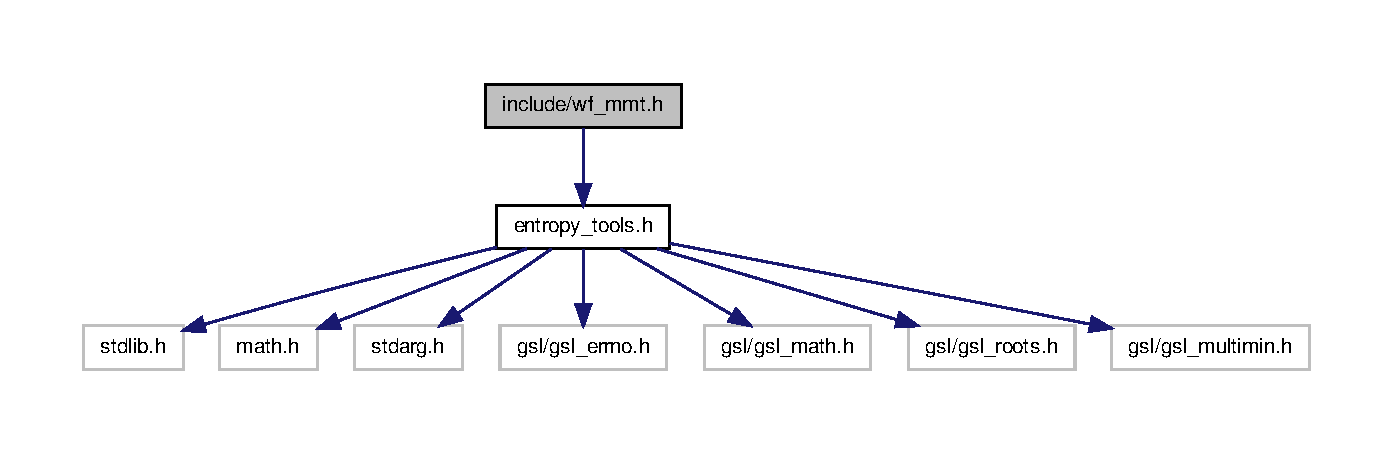
\includegraphics[width=350pt]{wf__mmt_8h__incl}
\end{center}
\end{figure}
\-This graph shows which files directly or indirectly include this file\-:
\nopagebreak
\begin{figure}[H]
\begin{center}
\leavevmode
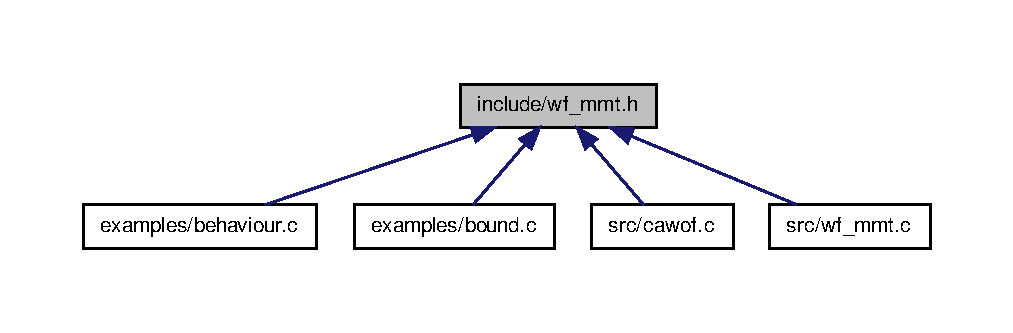
\includegraphics[width=350pt]{wf__mmt_8h__dep__incl}
\end{center}
\end{figure}


\subsection*{\-Functions}
\begin{DoxyCompactItemize}
\item 
double \hyperlink{wf__mmt_8h_afaaf2eaa35dcf780ab4405c3f6ce8707}{wf\-\_\-\-M\-M\-T} (const gsl\-\_\-vector $\ast$v, void $\ast$params)
\item 
double \hyperlink{wf__mmt_8h_a3d6e7472113ea6b9f6e05dd8800918e6}{\-Optimal\-\_\-wf\-\_\-\-M\-M\-T} (\hyperlink{structwf__params}{wf\-\_\-params} $\ast$params)
\end{DoxyCompactItemize}


\subsection{\-Detailed \-Description}
\-Library for calculation of \-M\-M\-T's \-Work \-Factor.  Definition in file \hyperlink{wf__mmt_8h}{wf\-\_\-mmt.\-h}.

\subsection{\-Function \-Documentation}

\hypertarget{wf__mmt_8h_afaaf2eaa35dcf780ab4405c3f6ce8707}{\index{wf\-\_\-mmt.\-h@{wf\-\_\-mmt.\-h}!wf\-\_\-\-M\-M\-T@{wf\-\_\-\-M\-M\-T}}
\index{wf\-\_\-\-M\-M\-T@{wf\-\_\-\-M\-M\-T}!wf_mmt.h@{wf\-\_\-mmt.\-h}}
\subsubsection[{wf\-\_\-\-M\-M\-T}]{\setlength{\rightskip}{0pt plus 5cm}double {\bf wf\-\_\-\-M\-M\-T} (
\begin{DoxyParamCaption}
\item[{const gsl\-\_\-vector $\ast$}]{v, }
\item[{void $\ast$}]{params}
\end{DoxyParamCaption}
)}}\label{wf__mmt_8h_afaaf2eaa35dcf780ab4405c3f6ce8707}

\-Work \-Factor of \-M\-M\-T's algorithm. Parameters l and p in v and k, w, \-N in params. 

\-Declaration at line 37 of file wf\-\_\-mmt.\-c.

\hypertarget{wf__mmt_8h_a3d6e7472113ea6b9f6e05dd8800918e6}{\index{wf\-\_\-mmt.\-h@{wf\-\_\-mmt.\-h}!\-Optimal\-\_\-wf\-\_\-\-M\-M\-T@{\-Optimal\-\_\-wf\-\_\-\-M\-M\-T}}
\index{\-Optimal\-\_\-wf\-\_\-\-M\-M\-T@{\-Optimal\-\_\-wf\-\_\-\-M\-M\-T}!wf_mmt.h@{wf\-\_\-mmt.\-h}}
\subsubsection[{\-Optimal\-\_\-wf\-\_\-\-M\-M\-T}]{\setlength{\rightskip}{0pt plus 5cm}double {\bf \-Optimal\-\_\-wf\-\_\-\-M\-M\-T} (
\begin{DoxyParamCaption}
\item[{{\bf wf\-\_\-params} $\ast$}]{params}
\end{DoxyParamCaption}
)}}\label{wf__mmt_8h_a3d6e7472113ea6b9f6e05dd8800918e6}

\-Optimal \-Work \-Factor of \-M\-M\-T's algorithm. Parameters k, w, \-N in params. \-It saves \-Optimal \-Parameters l and p in params.

\-Declaration at line 46 of file wf\-\_\-mmt.\-c.
\hypertarget{wf__nn_8h}{\section{include/wf\-\_\-nn.h \-File \-Reference}
\label{wf__nn_8h}\index{include/wf\-\_\-nn.\-h@{include/wf\-\_\-nn.\-h}}
}

\-Library for calculation of \-Nearest \-Neighboord's \-Work \-Factor.  

\subsection{Dependencies}

{\ttfamily \#include \char`\"{}entropy\-\_\-tools.\-h\char`\"{}}\*\\

\-Include dependency graph for wf\-\_\-nn.\-h\-:
\nopagebreak
\begin{figure}[H]
\begin{center}
\leavevmode
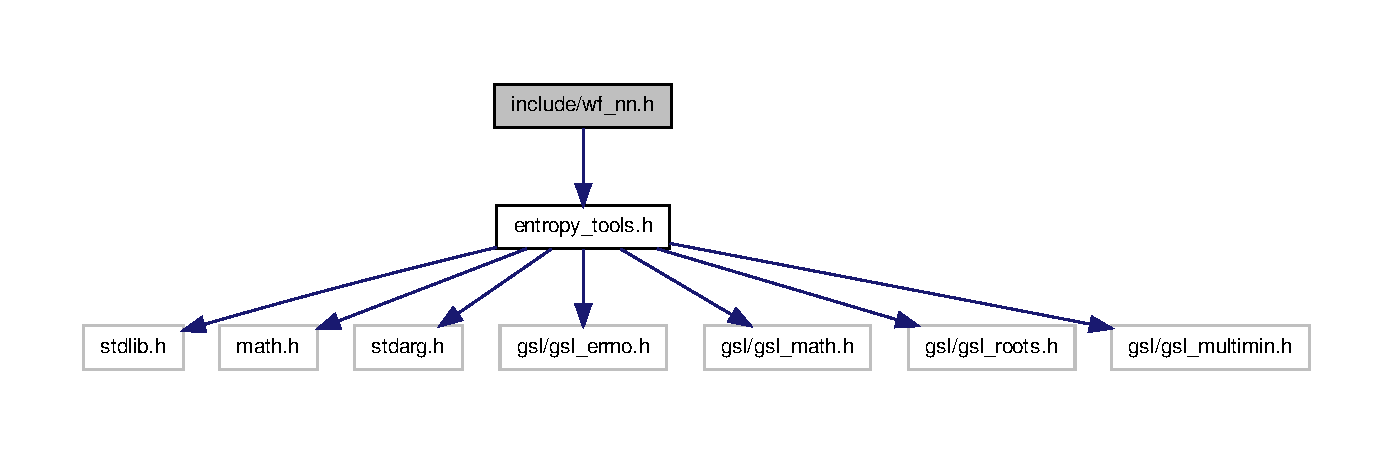
\includegraphics[width=350pt]{wf__nn_8h__incl}
\end{center}
\end{figure}
\-This graph shows which files directly or indirectly include this file\-:
\nopagebreak
\begin{figure}[H]
\begin{center}
\leavevmode
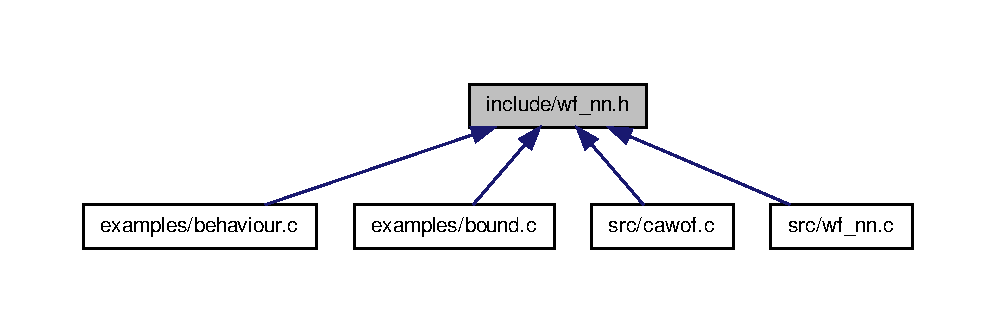
\includegraphics[width=350pt]{wf__nn_8h__dep__incl}
\end{center}
\end{figure}
  

\subsection*{\-Functions}
\begin{DoxyCompactItemize}
\item 
double \hyperlink{wf__nn_8h_a8dfefc665bca9dae6c43d725c23e6744}{wf\-\_\-\-N\-N} (double p2, void $\ast$paramslpp1)
\item 
double \hyperlink{wf__nn_8h_ad2f6d42b4446e77ad8c5d132f7535383}{\-Optimal\-\_\-wf\-\_\-\-N\-N\-\_\-p} (const gsl\-\_\-vector $\ast$v, void $\ast$params)
\item 
double \hyperlink{wf__nn_8h_aabe262ad8c85dbe0c434cba3463bd955}{\-Optimal\-\_\-wf\-\_\-\-N\-N} (\hyperlink{structwf__params}{wf\-\_\-params} $\ast$params)
\end{DoxyCompactItemize}


\subsection{\-Detailed \-Description}
\-Library for calculation of \-Nearest \-Neighboord's \-Work \-Factor. 

\-Definition in file \hyperlink{wf__nn_8h}{wf\-\_\-nn.\-h}.



\subsection{\-Function \-Documentation}

\hypertarget{wf__nn_8h_a8dfefc665bca9dae6c43d725c23e6744}{\index{wf\-\_\-nn.\-h@{wf\-\_\-nn.\-h}!wf\-\_\-\-N\-N@{wf\-\_\-\-N\-N}}
\index{wf\-\_\-\-N\-N@{wf\-\_\-\-N\-N}!wf_nn.h@{wf\-\_\-nn.\-h}}
\subsubsection[{wf\-\_\-\-N\-N}]{\setlength{\rightskip}{0pt plus 5cm}double {\bf wf\-\_\-\-N\-N} (
\begin{DoxyParamCaption}
\item[{double}]{p2, }
\item[{void $\ast$}]{paramslpp1}
\end{DoxyParamCaption}
)}}\label{wf__nn_8h_a8dfefc665bca9dae6c43d725c23e6744}

\-Work \-Factor of \-Nearest \-Neighbord's algorithm. Parameters k, w, \-N, l ,p, p1 in paramslpp1. 

\-Declaration at line 37 of file wf\-\_\-nn.\-h.

\hypertarget{wf__nn_8h_ad2f6d42b4446e77ad8c5d132f7535383}{\index{wf\-\_\-nn.\-h@{wf\-\_\-nn.\-h}!\-Optimal\-\_\-wf\-\_\-\-N\-N\-\_\-p@{\-Optimal\-\_\-wf\-\_\-\-N\-N\-\_\-p}}
\index{\-Optimal\-\_\-wf\-\_\-\-N\-N\-\_\-p@{\-Optimal\-\_\-wf\-\_\-\-N\-N\-\_\-p}!wf_nn.h@{wf\-\_\-nn.\-h}}
\subsubsection[{\-Optimal\-\_\-wf\-\_\-\-N\-N\-\_\-p}]{\setlength{\rightskip}{0pt plus 5cm}double {\bf \-Optimal\-\_\-wf\-\_\-\-N\-N\-\_\-p} (
\begin{DoxyParamCaption}
\item[{const gsl\-\_\-vector $\ast$}]{v, }
\item[{void $\ast$}]{params}
\end{DoxyParamCaption}
)}}\label{wf__nn_8h_ad2f6d42b4446e77ad8c5d132f7535383}

\-Optimal \-Work \-Factor of \-Nearest \-Neighbord's algorithm for l, p fixed. Parameters l and p in v and k, w, \-N in params. It saves \-Optimal \-Parameters p2 in paramslp ( p1 is chosen from l and p).

\-Declaration at line 48 of file wf\-\_\-nn.\-h.

\hypertarget{wf__nn_8h_aabe262ad8c85dbe0c434cba3463bd955}{\index{wf\-\_\-nn.\-h@{wf\-\_\-nn.\-h}!\-Optimal\-\_\-wf\-\_\-\-N\-N@{\-Optimal\-\_\-wf\-\_\-\-N\-N}}
\index{\-Optimal\-\_\-wf\-\_\-\-N\-N@{\-Optimal\-\_\-wf\-\_\-\-N\-N}!wf_nn.h@{wf\-\_\-nn.\-h}}
\subsubsection[{\-Optimal\-\_\-wf\-\_\-\-N\-N}]{\setlength{\rightskip}{0pt plus 5cm}double {\bf \-Optimal\-\_\-wf\-\_\-\-N\-N} (
\begin{DoxyParamCaption}
\item[{{\bf wf\-\_\-params} $\ast$}]{params}
\end{DoxyParamCaption}
)}}\label{wf__nn_8h_aabe262ad8c85dbe0c434cba3463bd955}

\-Optimal \-Work \-Factor of \-Nearest \-Neighbord's algorithm. Parameters k, w, \-N in params. \-It saves \-Optimal \-Parameters l, p, p1 and p2 in params. 

\-Declaration at line 58 of file wf\-\_\-nn.\-h.
\hypertarget{wf__prange_8h}{\section{include/wf\-\_\-prange.h \-File \-Reference}
\label{wf__prange_8h}\index{include/wf\-\_\-prange.\-h@{include/wf\-\_\-prange.\-h}}
}


\-Library for calculation of \-Prange's \-Work \-Factor.  

\subsection*{Dependencies}
{\ttfamily \#include \char`\"{}entropy\-\_\-tools.\-h\char`\"{}}\*\\

\-Include dependency graph for wf\-\_\-prange.\-h\-:\nopagebreak
\begin{figure}[H]
\begin{center}
\leavevmode
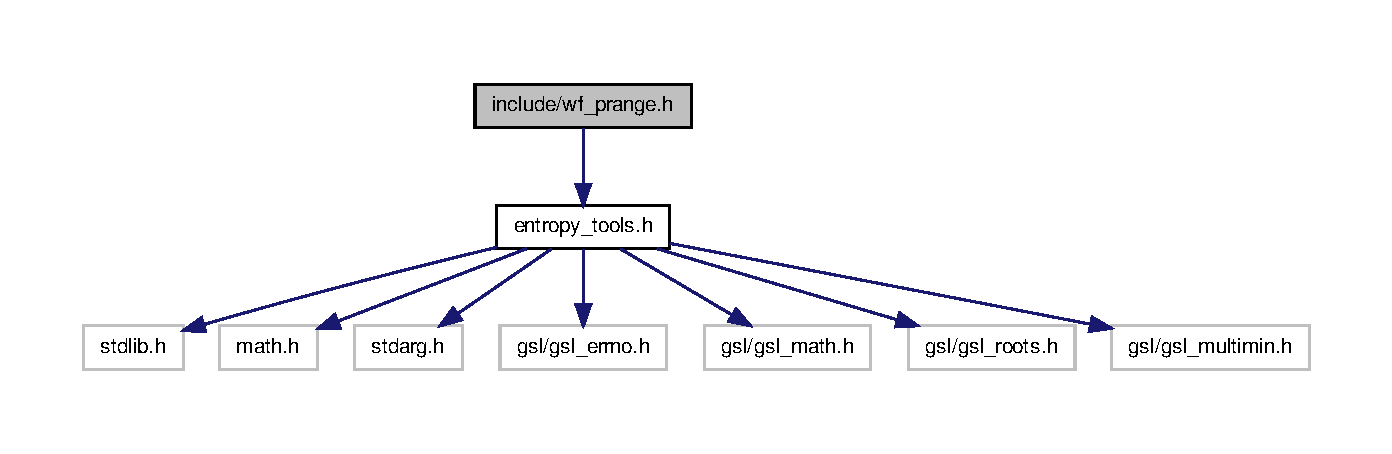
\includegraphics[width=350pt]{wf__prange_8h__incl}
\end{center}
\end{figure}
\-This graph shows which files directly or indirectly include this file\-:\nopagebreak
\begin{figure}[H]
\begin{center}
\leavevmode
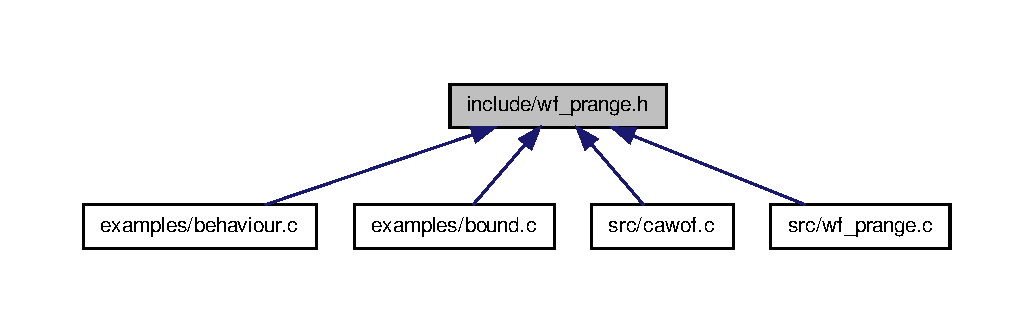
\includegraphics[width=350pt]{wf__prange_8h__dep__incl}
\end{center}
\end{figure}

\subsection*{\-Functions}
\begin{DoxyCompactItemize}
\item 
double \hyperlink{wf__prange_8h_aaab4db55369e553a26cfe4de8fb9ecb8}{wf\-\_\-\-Prange} (\hyperlink{structwf__params}{wf\-\_\-params} $\ast$params)
\end{DoxyCompactItemize}


\subsection{\-Detailed \-Description}
\-Library for calculation of \-Prange's \-Work \-Factor. 

\-Definition in file \hyperlink{wf__prange_8h}{wf\-\_\-prange.\-h}.



\subsection{\-Function \-Documentation}
\hypertarget{wf__prange_8h_aaab4db55369e553a26cfe4de8fb9ecb8}{\index{wf\-\_\-prange.\-h@{wf\-\_\-prange.\-h}!wf\-\_\-\-Prange@{wf\-\_\-\-Prange}}
\index{wf\-\_\-\-Prange@{wf\-\_\-\-Prange}!wf_prange.h@{wf\-\_\-prange.\-h}}
\subsubsection[{wf\-\_\-\-Prange}]{\setlength{\rightskip}{0pt plus 5cm}double {\bf wf\-\_\-\-Prange} (
\begin{DoxyParamCaption}
\item[{{\bf wf\-\_\-params} $\ast$}]{params}
\end{DoxyParamCaption}
)}}\label{wf__prange_8h_aaab4db55369e553a26cfe4de8fb9ecb8}

Work Factor of Prange's algorithm. 

\-Declaration at line 34 of file wf\-\_\-prange.\-h.


\hypertarget{wf__stern_8h}{\section{include/wf\-\_\-stern.h \-File \-Reference}
\label{wf__stern_8h}\index{include/wf\-\_\-stern.\-h@{include/wf\-\_\-stern.\-h}}
}

\-Library for calculation of Stern's \-Work \-Factor.  

\subsection*{Dependencies}
{\ttfamily \#include \char`\"{}entropy\-\_\-tools.\-h\char`\"{}}\*\\

\-Include dependency graph for wf\-\_\-stern.\-h\-:
\nopagebreak
\begin{figure}[H]
\begin{center}
\leavevmode
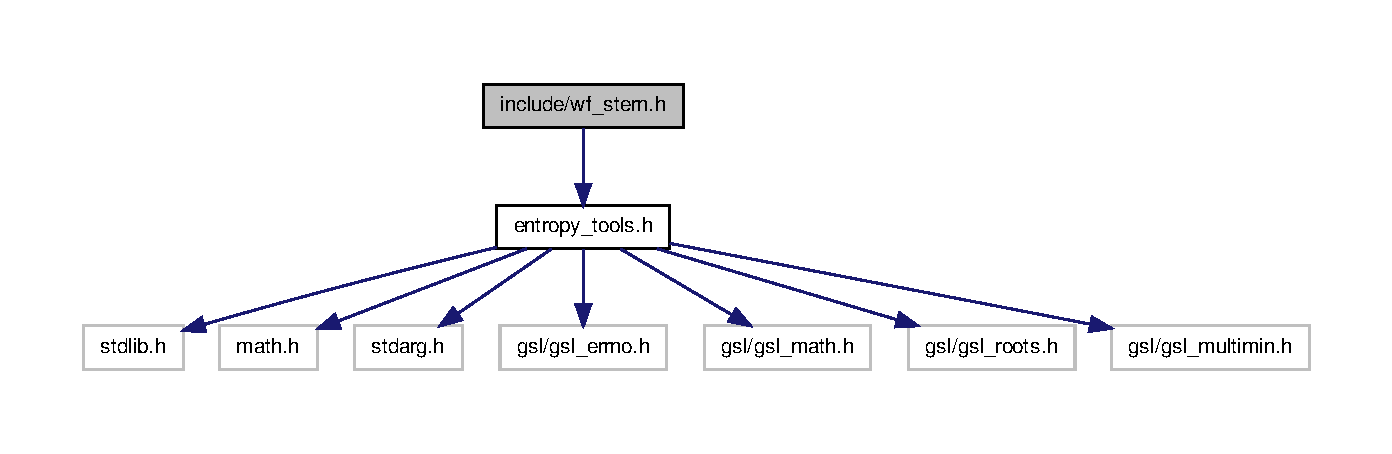
\includegraphics[width=350pt]{wf__stern_8h__incl}
\end{center}
\end{figure}
\-This graph shows which files directly or indirectly include this file\-:
\nopagebreak
\begin{figure}[H]
\begin{center}
\leavevmode
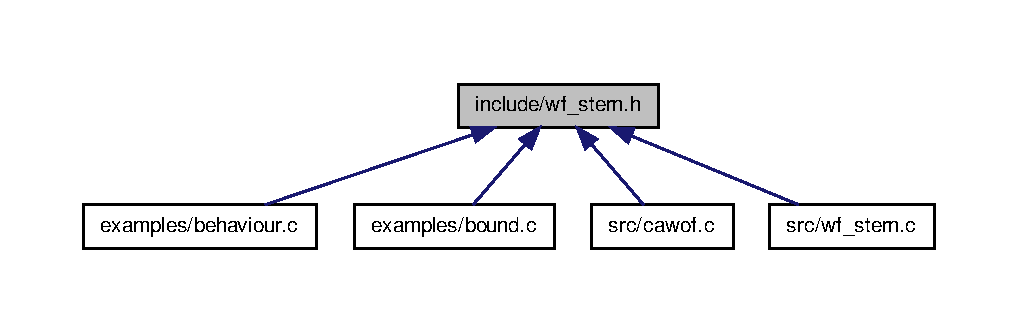
\includegraphics[width=350pt]{wf__stern_8h__dep__incl}
\end{center}
\end{figure}


\subsection*{\-Functions}
\begin{DoxyCompactItemize}
\item 
double \hyperlink{wf__stern_8h_a79ee922bb25d99869ec7f0fb94a109cc}{wf\-\_\-\-Stern} (const gsl\-\_\-vector $\ast$v, void $\ast$params)
\item 
double \hyperlink{wf__stern_8h_ad0f06aed633e1453adc6f85a5d1d35b2}{\-Optimal\-\_\-wf\-\_\-\-Stern} (\hyperlink{structwf__params}{wf\-\_\-params} $\ast$params)
\end{DoxyCompactItemize}


\subsection{\-Detailed \-Description}
\-Library for calculation of \-Nearest \-Neighboord's \-Work \-Factor. 

\-Definition in file \hyperlink{wf__stern_8h}{wf\-\_\-stern.\-h}.


\subsection{\-Function \-Documentation}

\hypertarget{wf__stern_8h_a79ee922bb25d99869ec7f0fb94a109cc}{\index{wf\-\_\-stern.\-h@{wf\-\_\-stern.\-h}!wf\-\_\-\-Stern@{wf\-\_\-\-Stern}}
\index{wf\-\_\-\-Stern@{wf\-\_\-\-Stern}!wf_stern.h@{wf\-\_\-stern.\-h}}
\subsubsection[{wf\-\_\-\-Stern}]{\setlength{\rightskip}{0pt plus 5cm}double {\bf wf\-\_\-\-Stern} (
\begin{DoxyParamCaption}
\item[{const gsl\-\_\-vector $\ast$}]{v, }
\item[{void $\ast$}]{params}
\end{DoxyParamCaption}
)}}\label{wf__stern_8h_a79ee922bb25d99869ec7f0fb94a109cc}

Work Factor of Stern's algorithm. Parameters l and p in v and k, w, N in params.

\-Declaration at line 37 of file wf\-\_\-stern.\-h.

\hypertarget{wf__stern_8h_ad0f06aed633e1453adc6f85a5d1d35b2}{\index{wf\-\_\-stern.\-h@{wf\-\_\-stern.\-h}!\-Optimal\-\_\-wf\-\_\-\-Stern@{\-Optimal\-\_\-wf\-\_\-\-Stern}}
\index{\-Optimal\-\_\-wf\-\_\-\-Stern@{\-Optimal\-\_\-wf\-\_\-\-Stern}!wf_stern.h@{wf\-\_\-stern.\-h}}
\subsubsection[{\-Optimal\-\_\-wf\-\_\-\-Stern}]{\setlength{\rightskip}{0pt plus 5cm}double {\bf \-Optimal\-\_\-wf\-\_\-\-Stern} (
\begin{DoxyParamCaption}
\item[{{\bf wf\-\_\-params} $\ast$}]{params}
\end{DoxyParamCaption}
)}}\label{wf__stern_8h_ad0f06aed633e1453adc6f85a5d1d35b2}


\-Optimal \-Work \-Factor of \-Stern's algorithm. Parameters k, w, \-N in params. \-It saves \-Optimal \-Parameters l and p in params.

\-Declaration at line 46 of file wf\-\_\-stern.\-h.


\hypertarget{bound__function_8c}{\section{src/bound\-\_\-function.c \-File \-Reference}
\label{bound__function_8c}\index{src/bound\-\_\-function.\-c@{src/bound\-\_\-function.\-c}}
}


\-Implementation of \hyperlink{bound__function_8h}{include/bound\-\_\-function.\-h}.  

\subsection*{Dependencies}

{\ttfamily \#include $<$bound\-\_\-function.\-h$>$}\*\\


\-Include dependency graph for bound\-\_\-function.\-c\-:\nopagebreak
\begin{figure}[H]
\begin{center}
\leavevmode
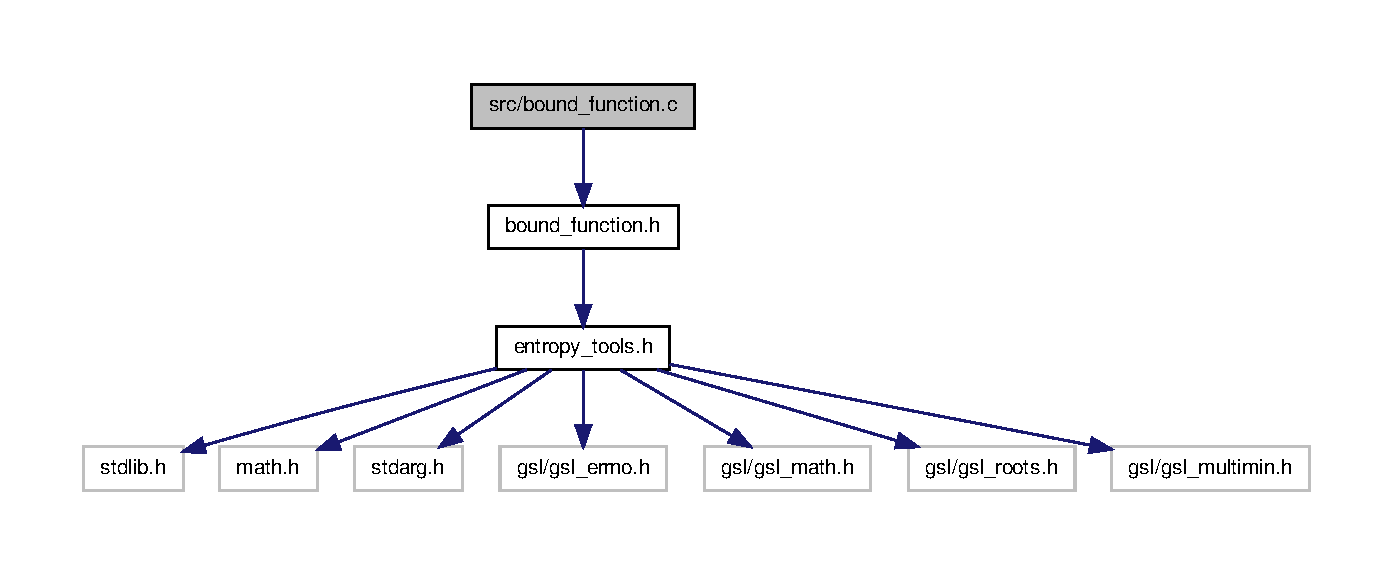
\includegraphics[width=350pt]{bound__function_8c__incl}
\end{center}
\end{figure}

\subsection*{\-Functions}
\begin{DoxyCompactItemize}
\item 
double \hyperlink{bound__function_8c_a3861f0ee3f0966eaa504ae6e96a5538b}{pp} (double l, \hyperlink{structwf__params}{wf\-\_\-params} $\ast$params)
\item 
double \hyperlink{bound__function_8c_ab8ab549d22869ed81b9eb0aece1bcbee}{dif\-\_\-pp} (double l, void $\ast$params)
\item 
double \hyperlink{bound__function_8c_adae35caf78299b2d048dc0d215ee1dc5}{pp\-\_\-df} (double l, \hyperlink{structwf__params}{wf\-\_\-params} $\ast$params)
\item 
double \hyperlink{bound__function_8c_a3af48831cb33dc02f5f72632592c8fc5}{reduced\-\_\-\-Ba} (double l, \hyperlink{structwf__params}{wf\-\_\-params} $\ast$params)
\item 
double \hyperlink{bound__function_8c_a18b7d91851ce5a2f94da2cb6ed20bc76}{reduced\-\_\-\-Ba\-\_\-df} (double l, void $\ast$params)
\item 
double \hyperlink{bound__function_8c_ae39e0703a1b025b97620c2fe2a17aed9}{l\-\_\-max} (\hyperlink{structwf__params}{wf\-\_\-params} $\ast$params)
\item 
double \hyperlink{bound__function_8c_a545abfeb71c0648db0a91dfa3e345e57}{\-Optimal\-\_\-reduced\-\_\-\-Ba} (\hyperlink{structwf__params}{wf\-\_\-params} $\ast$params)
\item 
double \hyperlink{bound__function_8c_ab965279f87e73cd3620cb491983ca3c4}{dif\-\_\-\-Optimal\-\_\-reduced\-\_\-\-Ba} (double a, void $\ast$params)
\item 
double \hyperlink{bound__function_8c_a806424a846d7c01ff8d78df2cf26c3ed}{find\-\_\-coefficient} (\hyperlink{structwf__params}{wf\-\_\-params} $\ast$params)
\end{DoxyCompactItemize}


\subsection{\-Detailed \-Description}
\-Implementation of \hyperlink{bound__function_8h}{include/bound\-\_\-function.\-h}. 

\-Definition in file \hyperlink{bound__function_8c}{bound\-\_\-function.\-c}.


\subsection{\-Function \-Documentation}

\hypertarget{bound__function_8c_a3861f0ee3f0966eaa504ae6e96a5538b}{\index{bound\-\_\-function.\-h@{bound\-\_\-function.\-h}!pp@{pp}}
\index{pp@{pp}!bound_function.h@{bound\-\_\-function.\-h}}
\subsubsection[{pp}]{\setlength{\rightskip}{0pt plus 5cm}double {\bf pp} (
\begin{DoxyParamCaption}
\item[{double}]{l, }
\item[{{\bf wf\-\_\-params} $\ast$}]{params}
\end{DoxyParamCaption}
)}}\label{bound__function_8c_a3861f0ee3f0966eaa504ae6e96a5538b}

\-Calculates the p such that 2$^\wedge$l=binomial(k+l,ap). 

\-Implementation at line 28 of file bound\-\_\-function.\-c.

\hypertarget{bound__function_8c_ab8ab549d22869ed81b9eb0aece1bcbee}{\index{bound\-\_\-function.\-h@{bound\-\_\-function.\-h}!dif\-\_\-pp@{dif\-\_\-pp}}
\index{dif\-\_\-pp@{dif\-\_\-pp}!bound_function.h@{bound\-\_\-function.\-h}}
\subsubsection[{dif\-\_\-pp}]{\setlength{\rightskip}{0pt plus 5cm}{\bf dif\-\_\-pp} (
\begin{DoxyParamCaption}
\item[{double}]{l, }
\item[{void $\ast$}]{params}
\end{DoxyParamCaption}
)}}\label{bound__function_8c_ab8ab549d22869ed81b9eb0aece1bcbee}


the diference pp(l,a)-\/w. Implementation at line 38 of file bound\-\_\-function.\-c.

\hypertarget{bound__function_8c_adae35caf78299b2d048dc0d215ee1dc5}{\index{bound\-\_\-function.\-h@{bound\-\_\-function.\-h}!pp\-\_\-df@{pp\-\_\-df}}
\index{pp\-\_\-df@{pp\-\_\-df}!bound_function.h@{bound\-\_\-function.\-h}}
\subsubsection[{pp\-\_\-df}]{\setlength{\rightskip}{0pt plus 5cm}{\bf pp\-\_\-df} (
\begin{DoxyParamCaption}
\item[{double}]{l, }
\item[{{\bf wf\-\_\-params} $\ast$}]{params}
\end{DoxyParamCaption}
)}}\label{bound__function_8c_adae35caf78299b2d048dc0d215ee1dc5}


\-Derivate of function pp. 

\-Implementation at line 44 of file bound\-\_\-function.\-c.

\hypertarget{bound__function_8c_a3af48831cb33dc02f5f72632592c8fc5}{\index{bound\-\_\-function.\-h@{bound\-\_\-function.\-h}!reduced\-\_\-\-Ba@{reduced\-\_\-\-Ba}}
\index{reduced\-\_\-\-Ba@{reduced\-\_\-\-Ba}!bound_function.h@{bound\-\_\-function.\-h}}
\subsubsection[{reduced\-\_\-\-Ba}]{\setlength{\rightskip}{0pt plus 5cm}double {\bf reduced\-\_\-\-Ba} (
\begin{DoxyParamCaption}
\item[{double}]{l, }
\item[{{\bf wf\-\_\-params} $\ast$}]{params}
\end{DoxyParamCaption}
)}}\label{bound__function_8c_a3af48831cb33dc02f5f72632592c8fc5}


\-Reduced version of \-Ba(l,p). This function will achieve the same minimum value of function \-Ba(l,p). 

\-Implementation at line 56 of file bound\-\_\-function.\-c.


\hypertarget{bound__function_8c_a18b7d91851ce5a2f94da2cb6ed20bc76}{\index{bound\-\_\-function.\-h@{bound\-\_\-function.\-h}!reduced\-\_\-\-Ba\-\_\-df@{reduced\-\_\-\-Ba\-\_\-df}}
\index{reduced\-\_\-\-Ba\-\_\-df@{reduced\-\_\-\-Ba\-\_\-df}!bound_function.h@{bound\-\_\-function.\-h}}
\subsubsection[{reduced\-\_\-\-Ba\-\_\-df}]{\setlength{\rightskip}{0pt plus 5cm}double {\bf reduced\-\_\-\-Ba\-\_\-df} (
\begin{DoxyParamCaption}
\item[{double}]{l, }
\item[{void $\ast$}]{params}
\end{DoxyParamCaption}
)}}\label{bound__function_8c_a18b7d91851ce5a2f94da2cb6ed20bc76}


\-Derivate of function reduced\-\_\-\-Ba. 

\-Declaration at line 67 of file bound\-\_\-function.\-h.

\hypertarget{bound__function_8c_ae39e0703a1b025b97620c2fe2a17aed9}{\index{bound\-\_\-function.\-h@{bound\-\_\-function.\-h}!l\-\_\-max@{l\-\_\-max}}
\index{l\-\_\-max@{l\-\_\-max}!bound_function.h@{bound\-\_\-function.\-h}}
\subsubsection[{l\-\_\-max}]{\setlength{\rightskip}{0pt plus 5cm}double {\bf l\-\_\-max} (
\begin{DoxyParamCaption}
\item[{{\bf wf\-\_\-params} $\ast$}]{params}
\end{DoxyParamCaption}
)}}\label{bound__function_8c_ae39e0703a1b025b97620c2fe2a17aed9}


\-Obtains the maximum value of l such \-Ba is calculable.

\-Implementation at line 82 of file bound\-\_\-function.\-c.


\hypertarget{bound__function_8c_a545abfeb71c0648db0a91dfa3e345e57}{\index{bound\-\_\-function.\-h@{bound\-\_\-function.\-h}!\-Optimal\-\_\-reduced\-\_\-\-Ba@{\-Optimal\-\_\-reduced\-\_\-\-Ba}}
\index{\-Optimal\-\_\-reduced\-\_\-\-Ba@{\-Optimal\-\_\-reduced\-\_\-\-Ba}!bound_function.h@{bound\-\_\-function.\-h}}
\subsubsection[{\-Optimal\-\_\-reduced\-\_\-\-Ba}]{\setlength{\rightskip}{0pt plus 5cm}double {\bf \-Optimal\-\_\-reduced\-\_\-\-Ba} (
\begin{DoxyParamCaption}
\item[{{\bf wf\-\_\-params} $\ast$}]{params}
\end{DoxyParamCaption}
)}}\label{bound__function_8c_a545abfeb71c0648db0a91dfa3e345e57}


\-Obtains the minimum value of \-Ba.

\-Implementation at line 131 of file bound\-\_\-function.\-c.



\hypertarget{bound__function_8c_ab965279f87e73cd3620cb491983ca3c4}{\index{bound\-\_\-function.\-h@{bound\-\_\-function.\-h}!dif\-\_\-\-Optimal\-\_\-reduced\-\_\-\-Ba@{dif\-\_\-\-Optimal\-\_\-reduced\-\_\-\-Ba}}
\index{dif\-\_\-\-Optimal\-\_\-reduced\-\_\-\-Ba@{dif\-\_\-\-Optimal\-\_\-reduced\-\_\-\-Ba}!bound_function.h@{bound\-\_\-function.\-h}}
\subsubsection[{dif\-\_\-\-Optimal\-\_\-reduced\-\_\-\-Ba}]{\setlength{\rightskip}{0pt plus 5cm}double {\bf dif\-\_\-\-Optimal\-\_\-reduced\-\_\-\-Ba} (
\begin{DoxyParamCaption}
\item[{double}]{a, }
\item[{void $\ast$}]{params}
\end{DoxyParamCaption}
)}}\label{bound__function_8c_ab965279f87e73cd3620cb491983ca3c4}


\-The difference \-Optimal\-\_\-reduced\-\_\-\-Ba -\/ workfactor.

\-Implementation at line 184 of file bound\-\_\-function.\-c.



\hypertarget{bound__function_8c_a806424a846d7c01ff8d78df2cf26c3ed}{\index{bound\-\_\-function.\-h@{bound\-\_\-function.\-h}!find\-\_\-coefficient@{find\-\_\-coefficient}}
\index{find\-\_\-coefficient@{find\-\_\-coefficient}!bound_function.h@{bound\-\_\-function.\-h}}
\subsubsection[{find\-\_\-coefficient}]{\setlength{\rightskip}{0pt plus 5cm}double {\bf find\-\_\-coefficient} (
\begin{DoxyParamCaption}
\item[{{\bf wf\-\_\-params} $\ast$}]{params}
\end{DoxyParamCaption}
)}}\label{bound__function_8c_a806424a846d7c01ff8d78df2cf26c3ed}


\-Find a such that reduced\-\_\-\-Ba\-\_\-min(a)=wf.

\-Implementation at line 195 of file bound\-\_\-function.\-c.
\hypertarget{cawof_8c}{\section{src/cawof.c \-File \-Reference}
\label{cawof_8c}\index{src/cawof.\-c@{src/cawof.\-c}}
}


\-Main program of calculation of \-Work \-Factor.  

\subsection*{Dependencies}

{\ttfamily \#include \char`\"{}cawof.\-h\char`\"{}}\*\\
{\ttfamily \#include $<$entropy\-\_\-tools.\-h$>$}\*\\
{\ttfamily \#include $<$wf\-\_\-prange.\-h$>$}\*\\
{\ttfamily \#include $<$wf\-\_\-stern.\-h$>$}\*\\
{\ttfamily \#include $<$wf\-\_\-dumer.\-h$>$}\*\\
{\ttfamily \#include $<$wf\-\_\-mmt.\-h$>$}\*\\
{\ttfamily \#include $<$wf\-\_\-bjmm.\-h$>$}\*\\
{\ttfamily \#include $<$wf\-\_\-nn.\-h$>$}\*\\
{\ttfamily \#include $<$stdbool.\-h$>$}\*\\
{\ttfamily \#include $<$stdlib.\-h$>$}\*\\
{\ttfamily \#include $<$stdio.\-h$>$}\*\\
{\ttfamily \#include $<$string.\-h$>$}\*\\
{\ttfamily \#include $<$getopt.\-h$>$}\*\\

Include dependency graph for cawof.\-c\-
\nopagebreak
\begin{figure}[H]
\begin{center}
\leavevmode
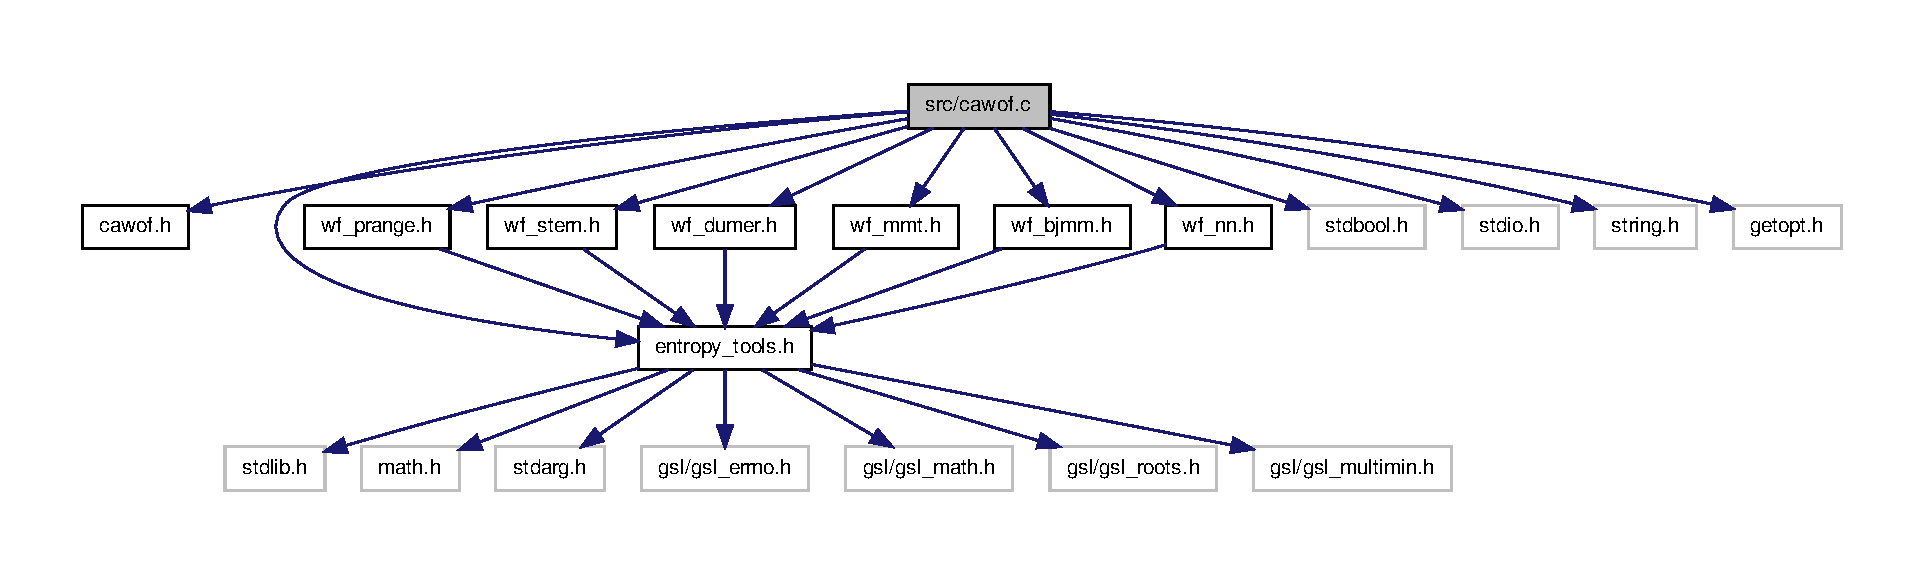
\includegraphics[width=350pt]{cawof_8c__incl}
\end{center}
\end{figure}

\subsection*{\-Functions}
\begin{DoxyCompactItemize}
\item 
void \hyperlink{cawof_8c_c0ddf1224851353fc92bfbff6f499fa97}{version} (void)
\item 
void \hyperlink{cawof_8c_r0ddf1224851353fc92bfbff6f499fa97}{usage} (int status)
\item 
int \hyperlink{cawof_8c_a0ddf1224851353fc92bfbff6f499fa97}{main} (int argc, char $\ast$argv\mbox{[}$\,$\mbox{]})

\end{DoxyCompactItemize}
\subsection*{\-Variables}
\begin{DoxyCompactItemize}
\item 
bool \hyperlink{cawof_8c_ab3f078684998b83967d507d0f453f454}{verbose}
\item 
bool \hyperlink{cawof_8c_ae4426f467d61ae456b95844d4d9c2dcd}{quiet}
\item 
bool \hyperlink{cawof_8c_a5eba86123523ed35aa48ccbd19d1b77a}{format}
\item 
\hyperlink{structwf__params}{wf\-\_\-params} \hyperlink{cawof_8c_aea89d30d6c8cc9ac79ded86e7f78d3ad}{wfp}
\item 
char \hyperlink{cawof_8c_ad7c92c302d8095e7b78a691e451ecf15}{algo} \mbox{[}20\mbox{]}
\item 
double($\ast$ \hyperlink{cawof_8c_a2254ed7d4ba79ef4b09f6801626aa1db}{wf\-\_\-algo} )(\hyperlink{structwf__params}{wf\-\_\-params} $\ast$)
\end{DoxyCompactItemize}


\subsection{\-Detailed \-Description}
Calculates of Work Factor of an ISD algorithm in the code rate and error rate. Default algorithm is BJMM, default code rate is 0.5 and defaut error rate is s Gilbert-Varshamov's bound. Available algorithms are PRANGE, STERN, DUMER, MMT, BJMM and NN.  

\-Definition in file \hyperlink{cawof_8c}{cawof.\-c}.

\subsection{\-Function \-Documentation}

\hypertarget{cawof_8c_c0ddf1224851353fc92bfbff6f499fa97}{\index{cawof.\-c@{cawof.\-c}!version@{version}}
\index{version@{version}!cawof.c@{cawof.\-c}}
\subsubsection[{version}]{\setlength{\rightskip}{0pt plus 5cm}void {\bf version} (
\begin{DoxyParamCaption}
\item[{void}]{}
\end{DoxyParamCaption}
)}}\label{cawof_8c_c0ddf1224851353fc92bfbff6f499fa97}

Print the version of program. 

\-Definition at line 56 of file cawof.\-c.


\hypertarget{cawof_8c_r0ddf1224851353fc92bfbff6f499fa97}{\index{cawof.\-c@{cawof.\-c}!usage@{usage}}
\index{usage@{usage}!cawof.c@{cawof.\-c}}
\subsubsection[{usage}]{\setlength{\rightskip}{0pt plus 5cm}void {\bf usage} (
\begin{DoxyParamCaption}
\item[{int}]{status}
\end{DoxyParamCaption}
)}}\label{cawof_8c_r0ddf1224851353fc92bfbff6f499fa97}

Print the help of program. 

\-Definition at line 68 of file cawof.\-c.

\hypertarget{cawof_8c_a0ddf1224851353fc92bfbff6f499fa97}{\index{cawof.\-c@{cawof.\-c}!main@{main}}
\index{main@{main}!cawof.c@{cawof.\-c}}
\subsubsection[{main}]{\setlength{\rightskip}{0pt plus 5cm}int {\bf main} (
\begin{DoxyParamCaption}
\item[{int}]{argc, }
\item[{char $\ast$}]{argv\mbox{[}$\,$\mbox{]}}
\end{DoxyParamCaption}
)}}\label{cawof_8c_a0ddf1224851353fc92bfbff6f499fa97}

Calculates of Work Factor of an ISD algorithm in the code rate and error rate. 

\-Definition at line 96 of file cawof.\-c.

\subsection{\-Variable \-Documentation}

\hypertarget{cawof_8c_ab3f078684998b83967d507d0f453f454}{\index{cawof.\-c@{cawof.\-c}!verbose@{verbose}}
\index{verbose@{verbose}!cawof.c@{cawof.\-c}}
\subsubsection[{verbose}]{\setlength{\rightskip}{0pt plus 5cm}bool {\bf verbose}}}\label{cawof_8c_ab3f078684998b83967d507d0f453f454}

Decides if the program prints the values of optimal parameters for the algorithm. 

\-Definition at line 46 of file cawof.\-c.

\hypertarget{cawof_8c_ae4426f467d61ae456b95844d4d9c2dcd}{\index{cawof.\-c@{cawof.\-c}!quiet@{quiet}}
\index{quiet@{quiet}!cawof.c@{cawof.\-c}}
\subsubsection[{quiet}]{\setlength{\rightskip}{0pt plus 5cm}bool {\bf quiet}}}\label{cawof_8c_ae4426f467d61ae456b95844d4d9c2dcd}


Decides if the program prints explanation of results. 

\-Definition at line 46 of file cawof.\-c.


\hypertarget{cawof_8c_a5eba86123523ed35aa48ccbd19d1b77a}{\index{cawof.\-c@{cawof.\-c}!format@{format}}
\index{format@{format}!cawof.c@{cawof.\-c}}
\subsubsection[{format}]{\setlength{\rightskip}{0pt plus 5cm}bool {\bf format}}}\label{cawof_8c_a5eba86123523ed35aa48ccbd19d1b77a}


Decides if the work factor is expressed in terms of w or n. 

\-Definition at line 46 of file cawof.\-c.

\hypertarget{cawof_8c_aea89d30d6c8cc9ac79ded86e7f78d3ad}{\index{cawof.\-c@{cawof.\-c}!wfp@{wfp}}
\index{wfp@{wfp}!cawof.c@{cawof.\-c}}
\subsubsection[{wfp}]{\setlength{\rightskip}{0pt plus 5cm}{\bf wf\-\_\-params} {\bf wfp}}}\label{cawof_8c_aea89d30d6c8cc9ac79ded86e7f78d3ad}


It contains the parameters of coding algorithm. 

\-Definition at line 47 of file cawof.\-c.

\hypertarget{cawof_8c_ad7c92c302d8095e7b78a691e451ecf15}{\index{cawof.\-c@{cawof.\-c}!algo@{algo}}
\index{algo@{algo}!cawof.c@{cawof.\-c}}
\subsubsection[{algo}]{\setlength{\rightskip}{0pt plus 5cm}char {\bf algo}\mbox{[}20\mbox{]}}}\label{cawof_8c_ad7c92c302d8095e7b78a691e451ecf15}

It saves the name of algorithm to analyze.

\-Definition at line 48 of file cawof.\-c.

\hypertarget{cawof_8c_a2254ed7d4ba79ef4b09f6801626aa1db}{\index{cawof.\-c@{cawof.\-c}!wf\-\_\-algo@{wf\-\_\-algo}}
\index{wf\-\_\-algo@{wf\-\_\-algo}!cawof.c@{cawof.\-c}}
\subsubsection[{wf\-\_\-algo}]{\setlength{\rightskip}{0pt plus 5cm}double($\ast$  {\bf wf\-\_\-algo})({\bf wf\-\_\-params} $\ast$)}}\label{cawof_8c_a2254ed7d4ba79ef4b09f6801626aa1db}


It contains the optimization function to use. 

\-Definition at line 49 of file cawof.\-c.
\hypertarget{cawof_8h}{\section{src/cawof.h \-File \-Reference}
\label{cawof_8h}\index{src/cawof.\-h@{src/cawof.\-h}}
}

\-Definiton of constants for the principal program.  
\subsection*{Dependencies}

\-This graph shows which files directly or indirectly include this file\-:\nopagebreak
\begin{figure}[H]
\begin{center}
\leavevmode
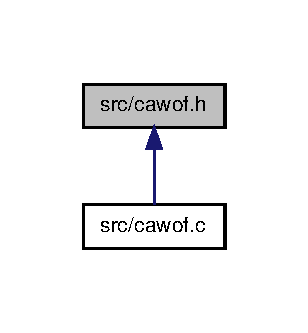
\includegraphics[width=148pt]{cawof_8h__dep__incl}
\end{center}
\end{figure}

\subsection*{\-Defines}
\begin{DoxyCompactItemize}
\item 
\#define \hyperlink{cawof_8h_a44493dbd21a529ec6fdb2da73a35ac70}{\-P\-R\-O\-G\-\_\-\-N\-A\-M\-E}~\char`\"{}\-Ca\-Wo\-F\char`\"{}
\item 
\#define \hyperlink{cawof_8h_a50ef2e611dcbc13c41a2bb2556009c61}{\-P\-R\-O\-G\-\_\-\-V\-E\-R\-S\-I\-O\-N}~1
\item 
\#define \hyperlink{cawof_8h_ace7590a102aed635f31ae83217dc0900}{\-P\-R\-O\-G\-\_\-\-S\-U\-B\-V\-E\-R\-S\-I\-O\-N}~0
\item 
\#define \hyperlink{cawof_8h_a794b131c8e431a71c4b92a90c8569ca2}{\-P\-R\-O\-G\-\_\-\-R\-E\-V\-I\-S\-I\-O\-N}~0
\end{DoxyCompactItemize}


\subsection{\-Detailed \-Description}
\-Definiton of constants for the principal program. 

\-Definition in file \hyperlink{cawof_8h}{cawof.\-h}.

\subsection{\-Define \-Documentation}
\hypertarget{cawof_8h_a44493dbd21a529ec6fdb2da73a35ac70}{\index{cawof.\-h@{cawof.\-h}!\-P\-R\-O\-G\-\_\-\-N\-A\-M\-E@{\-P\-R\-O\-G\-\_\-\-N\-A\-M\-E}}
\index{\-P\-R\-O\-G\-\_\-\-N\-A\-M\-E@{\-P\-R\-O\-G\-\_\-\-N\-A\-M\-E}!cawof.h@{cawof.\-h}}
\subsubsection[{\-P\-R\-O\-G\-\_\-\-N\-A\-M\-E}]{\setlength{\rightskip}{0pt plus 5cm}\#define {\bf \-P\-R\-O\-G\-\_\-\-N\-A\-M\-E}~\char`\"{}\-Ca\-Wo\-F\char`\"{}}}\label{cawof_8h_a44493dbd21a529ec6fdb2da73a35ac70}

Definition at line 30 of file cawof.\-h.

\hypertarget{cawof_8h_a50ef2e611dcbc13c41a2bb2556009c61}{\index{cawof.\-h@{cawof.\-h}!\-P\-R\-O\-G\-\_\-\-V\-E\-R\-S\-I\-O\-N@{\-P\-R\-O\-G\-\_\-\-V\-E\-R\-S\-I\-O\-N}}
\index{\-P\-R\-O\-G\-\_\-\-V\-E\-R\-S\-I\-O\-N@{\-P\-R\-O\-G\-\_\-\-V\-E\-R\-S\-I\-O\-N}!cawof.h@{cawof.\-h}}
\subsubsection[{\-P\-R\-O\-G\-\_\-\-V\-E\-R\-S\-I\-O\-N}]{\setlength{\rightskip}{0pt plus 5cm}\#define {\bf \-P\-R\-O\-G\-\_\-\-V\-E\-R\-S\-I\-O\-N}~1}}\label{cawof_8h_a50ef2e611dcbc13c41a2bb2556009c61}

\-Definition at line 32 of file cawof.\-h.

\hypertarget{cawof_8h_ace7590a102aed635f31ae83217dc0900}{\index{cawof.\-h@{cawof.\-h}!\-P\-R\-O\-G\-\_\-\-S\-U\-B\-V\-E\-R\-S\-I\-O\-N@{\-P\-R\-O\-G\-\_\-\-S\-U\-B\-V\-E\-R\-S\-I\-O\-N}}
\index{\-P\-R\-O\-G\-\_\-\-S\-U\-B\-V\-E\-R\-S\-I\-O\-N@{\-P\-R\-O\-G\-\_\-\-S\-U\-B\-V\-E\-R\-S\-I\-O\-N}!cawof.h@{cawof.\-h}}
\subsubsection[{\-P\-R\-O\-G\-\_\-\-S\-U\-B\-V\-E\-R\-S\-I\-O\-N}]{\setlength{\rightskip}{0pt plus 5cm}\#define {\bf \-P\-R\-O\-G\-\_\-\-S\-U\-B\-V\-E\-R\-S\-I\-O\-N}~0}}\label{cawof_8h_ace7590a102aed635f31ae83217dc0900}

Definition at line 33 of file cawof.\-h.


\hypertarget{cawof_8h_a794b131c8e431a71c4b92a90c8569ca2}{\index{cawof.\-h@{cawof.\-h}!\-P\-R\-O\-G\-\_\-\-R\-E\-V\-I\-S\-I\-O\-N@{\-P\-R\-O\-G\-\_\-\-R\-E\-V\-I\-S\-I\-O\-N}}
\index{\-P\-R\-O\-G\-\_\-\-R\-E\-V\-I\-S\-I\-O\-N@{\-P\-R\-O\-G\-\_\-\-R\-E\-V\-I\-S\-I\-O\-N}!cawof.h@{cawof.\-h}}
\subsubsection[{\-P\-R\-O\-G\-\_\-\-R\-E\-V\-I\-S\-I\-O\-N}]{\setlength{\rightskip}{0pt plus 5cm}\#define {\bf \-P\-R\-O\-G\-\_\-\-R\-E\-V\-I\-S\-I\-O\-N}~0}}\label{cawof_8h_a794b131c8e431a71c4b92a90c8569ca2}

Definition at line 34 of file cawof.\-h.
\hypertarget{entropy__tools_8c}{\section{src/entropy\-\_\-tools.c \-File \-Reference}
\label{entropy__tools_8c}\index{src/entropy\-\_\-tools.\-c@{src/entropy\-\_\-tools.\-c}}
}

\-Implementation of \hyperlink{entropy__tools_8h}{include/entropy\-\_\-tools.\-h}.  

\subsection*{Dependencies}

{\ttfamily \#include $<$entropy\-\_\-tools.\-h$>$}\*\\

Include dependency graph for entropy\-\_\-tools.\-c\-:\nopagebreak
\begin{figure}[H]
\begin{center}
\leavevmode
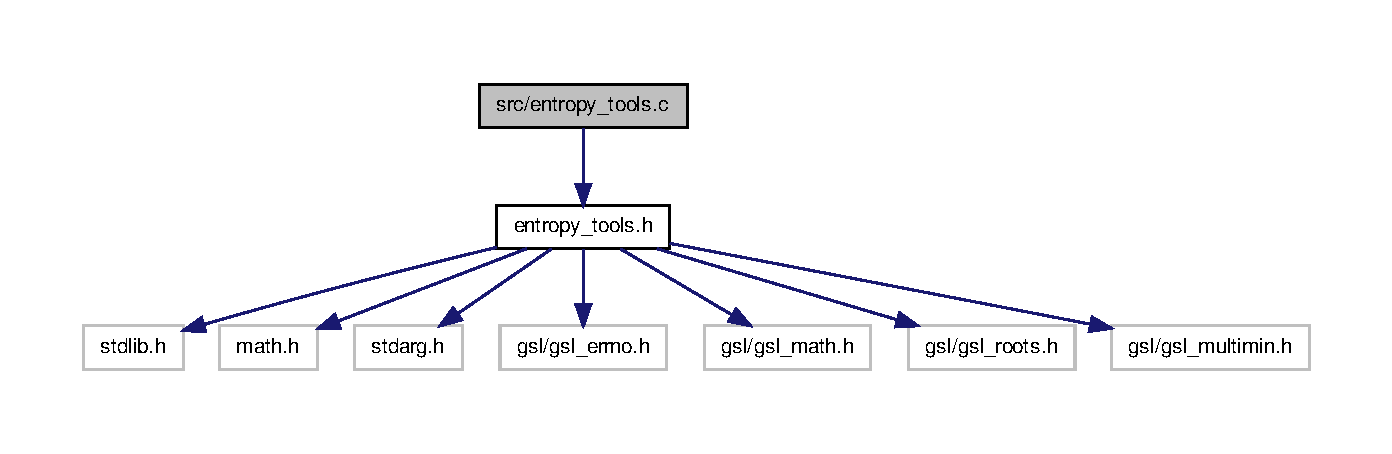
\includegraphics[width=350pt]{entropy__tools_8c__incl}
\end{center}
\end{figure}


\subsection*{\-Functions}
\begin{DoxyCompactItemize}
\item 
double \hyperlink{entropy__tools_8c_af66cf5e05f6372e2f5698c1fd5f53a13}{max} (int num,...)
\item 
double \hyperlink{entropy__tools_8c_a2f8edc4561e9744ed4233b205fa7ec32}{min} (double x, double y)
\item 
double \hyperlink{entropy__tools_8c_a1c878e40e9fb5c8aabfcc699f073c6b3}{entropy} (double x)
\item 
double \hyperlink{entropy__tools_8c_a5e0594a7998f7a5a8ee1ba6a47ac1833}{binomial} (double x, double y)
\item 
double \hyperlink{entropy__tools_8c_abc8201a1eb0c80331fc4e86179313e30}{dif\-\_\-entropy} (double x, void $\ast$params)
\item 
double \hyperlink{entropy__tools_8c_a13508874928cb281385d71441ce19338}{entropy\-\_\-df} (double x, void $\ast$params)
\item 
void \hyperlink{entropy__tools_8c_afb5ad221506034a3e0d1763c42730bdf}{entropy\-\_\-fdf} (double x, void $\ast$params, double $\ast$y, double $\ast$dy)
\item 
double \hyperlink{entropy__tools_8c_a682ad4530749e13582d63bfab2aada60}{entropy\-\_\-inverse} (double y)
\end{DoxyCompactItemize}


\subsection{\-Detailed \-Description}
\-Implementation of \hyperlink{entropy__tools_8h}{include/entropy\-\_\-tools.\-h}. 

\-Definition in file \hyperlink{entropy__tools_8c}{entropy\-\_\-tools.\-c}.

\subsection{\-Function \-Documentation}


\hypertarget{entropy__tools_8c_af66cf5e05f6372e2f5698c1fd5f53a13}{\index{entropy\-\_\-tools.\-c@{entropy\-\_\-tools.\-c}!max@{max}}
\index{max@{max}!entropy_tools.c@{entropy\-\_\-tools.\-c}}
\subsubsection[{max}]{\setlength{\rightskip}{0pt plus 5cm}double {\bf max} (
\begin{DoxyParamCaption}
\item[{int}]{num, }
\item[{}]{...}
\end{DoxyParamCaption}
)}}\label{entropy__tools_8c_af66cf5e05f6372e2f5698c1fd5f53a13}


\-Maximum of num double values. 

\-Implementation at line 28 of file entropy\-\_\-tools.\-c.

\hypertarget{entropy__tools_8c_a2f8edc4561e9744ed4233b205fa7ec32}{\index{entropy\-\_\-tools.\-c@{entropy\-\_\-tools.\-c}!min@{min}}
\index{min@{min}!entropy_tools.c@{entropy\-\_\-tools.\-c}}
\subsubsection[{min}]{\setlength{\rightskip}{0pt plus 5cm}double {\bf min} (
\begin{DoxyParamCaption}
\item[{double}]{x, }
\item[{double}]{y}
\end{DoxyParamCaption}
)}}\label{entropy__tools_8c_a2f8edc4561e9744ed4233b205fa7ec32}

\-Minimum of two double values. 

\-Implementation at line 49 of file entropy\-\_\-tools.\-c.

\hypertarget{entropy__tools_8c_a1c878e40e9fb5c8aabfcc699f073c6b3}{\index{entropy\-\_\-tools.\-c@{entropy\-\_\-tools.\-c}!entropy@{entropy}}
\index{entropy@{entropy}!entropy_tools.c@{entropy\-\_\-tools.\-c}}
\subsubsection[{entropy}]{\setlength{\rightskip}{0pt plus 5cm}double {\bf entropy} (
\begin{DoxyParamCaption}
\item[{double}]{x}
\end{DoxyParamCaption}
)}}\label{entropy__tools_8c_a1c878e40e9fb5c8aabfcc699f073c6b3}


\-This function calculates the (binary) entropy. 

\-Implementation at line 57 of file entropy\-\_\-tools.\-c.

\hypertarget{entropy__tools_8c_a5e0594a7998f7a5a8ee1ba6a47ac1833}{\index{entropy\-\_\-tools.\-c@{entropy\-\_\-tools.\-c}!binomial@{binomial}}
\index{binomial@{binomial}!entropy_tools.c@{entropy\-\_\-tools.\-c}}
\subsubsection[{binomial}]{\setlength{\rightskip}{0pt plus 5cm}double {\bf binomial} (
\begin{DoxyParamCaption}
\item[{double}]{x, }
\item[{double}]{y}
\end{DoxyParamCaption}
)}}\label{entropy__tools_8c_a5e0594a7998f7a5a8ee1ba6a47ac1833}


\-This function approximates \-Binomial coefficient by entropy function. 

\-Implementation at line 65 of file entropy\-\_\-tools.\-c.

\hypertarget{entropy__tools_8c_abc8201a1eb0c80331fc4e86179313e30}{\index{entropy\-\_\-tools.\-c@{entropy\-\_\-tools.\-c}!dif\-\_\-entropy@{dif\-\_\-entropy}}
\index{dif\-\_\-entropy@{dif\-\_\-entropy}!entropy_tools.c@{entropy\-\_\-tools.\-c}}
\subsubsection[{dif\-\_\-entropy}]{\setlength{\rightskip}{0pt plus 5cm}double {\bf dif\-\_\-entropy} (
\begin{DoxyParamCaption}
\item[{double}]{x, }
\item[{void $\ast$}]{params}
\end{DoxyParamCaption}
)}}\label{entropy__tools_8c_abc8201a1eb0c80331fc4e86179313e30}


\-The diference entropy(x)-\/params. 

\-Implementation at line 73 of file entropy\-\_\-tools.\-c.


\hypertarget{entropy__tools_8c_a13508874928cb281385d71441ce19338}{\index{entropy\-\_\-tools.\-c@{entropy\-\_\-tools.\-c}!entropy\-\_\-df@{entropy\-\_\-df}}
\index{entropy\-\_\-df@{entropy\-\_\-df}!entropy_tools.c@{entropy\-\_\-tools.\-c}}
\subsubsection[{entropy\-\_\-df}]{\setlength{\rightskip}{0pt plus 5cm}double {\bf entropy\-\_\-df} (
\begin{DoxyParamCaption}
\item[{double}]{x, }
\item[{void $\ast$}]{params}
\end{DoxyParamCaption}
)}}\label{entropy__tools_8c_a13508874928cb281385d71441ce19338}


\-Derivate of entropy function. 

\-Implementation at line 82 of file entropy\-\_\-tools.\-c.

\hypertarget{entropy__tools_8c_afb5ad221506034a3e0d1763c42730bdf}{\index{entropy\-\_\-tools.\-c@{entropy\-\_\-tools.\-c}!entropy\-\_\-fdf@{entropy\-\_\-fdf}}
\index{entropy\-\_\-fdf@{entropy\-\_\-fdf}!entropy_tools.c@{entropy\-\_\-tools.\-c}}
\subsubsection[{entropy\-\_\-fdf}]{\setlength{\rightskip}{0pt plus 5cm}void {\bf entropy\-\_\-fdf} (
\begin{DoxyParamCaption}
\item[{double}]{x, }
\item[{void $\ast$}]{params, }
\item[{double $\ast$}]{y, }
\item[{double $\ast$}]{dy}
\end{DoxyParamCaption}
)}}\label{entropy__tools_8c_afb5ad221506034a3e0d1763c42730bdf}


\-Obtains the dif\-\_\-entropy function and its derivate.

\-Implementation at line 88 of file entropy\-\_\-tools.\-c.

\hypertarget{entropy__tools_8c_a682ad4530749e13582d63bfab2aada60}{\index{entropy\-\_\-tools.\-c@{entropy\-\_\-tools.\-c}!entropy\-\_\-inverse@{entropy\-\_\-inverse}}
\index{entropy\-\_\-inverse@{entropy\-\_\-inverse}!entropy_tools.c@{entropy\-\_\-tools.\-c}}
\subsubsection[{entropy\-\_\-inverse}]{\setlength{\rightskip}{0pt plus 5cm}double {\bf entropy\-\_\-inverse} (
\begin{DoxyParamCaption}
\item[{double}]{y}
\end{DoxyParamCaption}
)}}\label{entropy__tools_8c_a682ad4530749e13582d63bfab2aada60}


\-Obtains the inverse of entropy function and return a real in \mbox{[}0,0.\-5\mbox{]}

\-Implementation at line 96 of file entropy\-\_\-tools.\-c.
\hypertarget{wf__bjmm_8c}{\section{src/wf\-\_\-bjmm.c \-File \-Reference}
\label{wf__bjmm_8c}\index{src/wf\-\_\-bjmm.\-c@{src/wf\-\_\-bjmm.\-c}}
}


\-Implementation of \hyperlink{wf__bjmm_8h}{include/wf\-\_\-bjmm.\-h}.  
\subsection*{Dependencies}
{\ttfamily \#include $<$wf\-\_\-bjmm.\-h$>$}\*\\

\-Include dependency graph for wf\-\_\-bjmm.\-c\-:\nopagebreak
\begin{figure}[H]
\begin{center}
\leavevmode
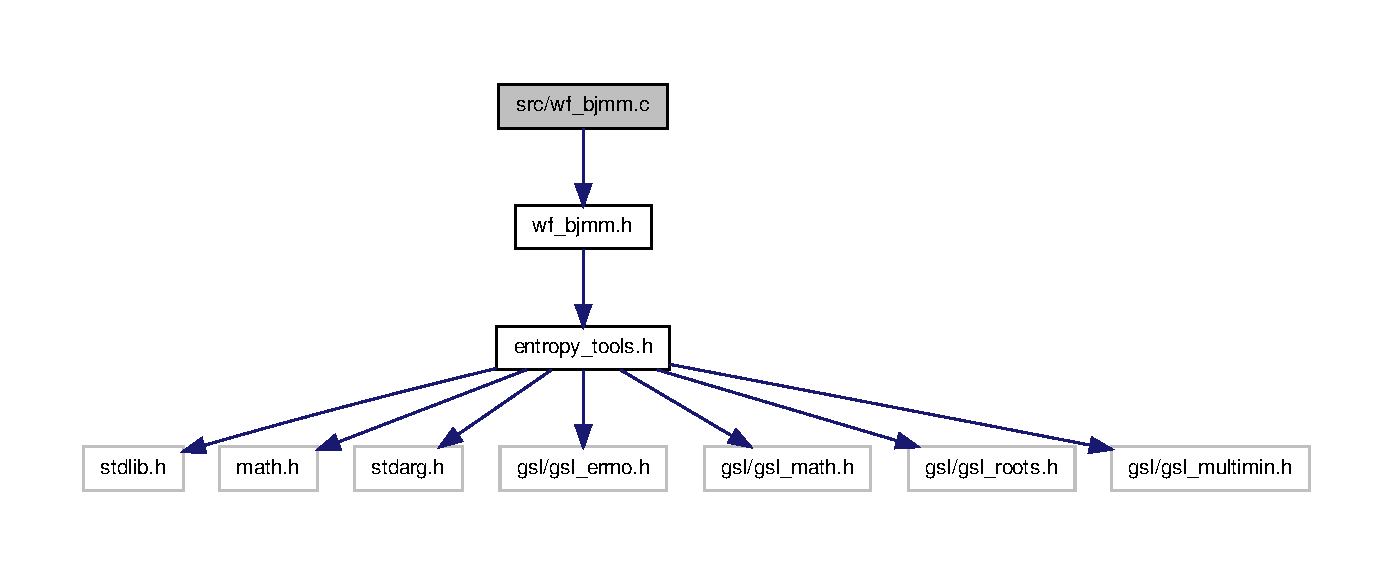
\includegraphics[width=350pt]{wf__bjmm_8c__incl}
\end{center}
\end{figure}

\subsection*{\-Functions}
\begin{DoxyCompactItemize}
\item 
double \hyperlink{wf__bjmm_8c_afb4fca4c10e792952c64c8d712f44947}{wf\-\_\-\-B\-J\-M\-M} (const gsl\-\_\-vector $\ast$v, void $\ast$paramslp)
\item 
double \hyperlink{wf__bjmm_8c_a57582cc5476f2d16374afc1052b5a492}{\-Optimal\-\_\-wf\-\_\-\-B\-J\-M\-M\-\_\-p12} (const gsl\-\_\-vector $\ast$vv, void $\ast$params)
\item 
double \hyperlink{wf__bjmm_8c_aa1a2efb0ac81db558018172e12d0958d}{\-Optimal\-\_\-wf\-\_\-\-B\-J\-M\-M} (\hyperlink{structwf__params}{wf\-\_\-params} $\ast$params)
\end{DoxyCompactItemize}


\subsection{\-Detailed \-Description}
\-Implementation of \hyperlink{wf__bjmm_8h}{include/wf\-\_\-bjmm.\-h}.

\-Definition in file \hyperlink{wf__bjmm_8c}{wf\-\_\-bjmm.\-c}.

\subsection{\-Function \-Documentation}

\hypertarget{wf__bjmm_8c_afb4fca4c10e792952c64c8d712f44947}{\index{wf\-\_\-bjmm.\-c@{wf\-\_\-bjmm.\-c}!wf\-\_\-\-B\-J\-M\-M@{wf\-\_\-\-B\-J\-M\-M}}
\index{wf\-\_\-\-B\-J\-M\-M@{wf\-\_\-\-B\-J\-M\-M}!wf_bjmm.c@{wf\-\_\-bjmm.\-c}}
\subsubsection[{wf\-\_\-\-B\-J\-M\-M}]{\setlength{\rightskip}{0pt plus 5cm}double {\bf wf\-\_\-\-B\-J\-M\-M} (
\begin{DoxyParamCaption}
\item[{const gsl\-\_\-vector $\ast$}]{v, }
\item[{void $\ast$}]{paramslp}
\end{DoxyParamCaption}
)}}\label{wf__bjmm_8c_afb4fca4c10e792952c64c8d712f44947}

Work Factor of BJMM's algorithm. Parameters p1 and p2 in  v and k, w, N, l ,p in paramslp.

\-Implementation at line 29 of file wf\-\_\-bjmm.\-c.

\hypertarget{wf__bjmm_8c_a57582cc5476f2d16374afc1052b5a492}{\index{wf\-\_\-bjmm.\-c@{wf\-\_\-bjmm.\-c}!\-Optimal\-\_\-wf\-\_\-\-B\-J\-M\-M\-\_\-p12@{\-Optimal\-\_\-wf\-\_\-\-B\-J\-M\-M\-\_\-p12}}
\index{\-Optimal\-\_\-wf\-\_\-\-B\-J\-M\-M\-\_\-p12@{\-Optimal\-\_\-wf\-\_\-\-B\-J\-M\-M\-\_\-p12}!wf_bjmm.c@{wf\-\_\-bjmm.\-c}}
\subsubsection[{\-Optimal\-\_\-wf\-\_\-\-B\-J\-M\-M\-\_\-p12}]{\setlength{\rightskip}{0pt plus 5cm}double {\bf \-Optimal\-\_\-wf\-\_\-\-B\-J\-M\-M\-\_\-p12} (
\begin{DoxyParamCaption}
\item[{const gsl\-\_\-vector $\ast$}]{vv, }
\item[{void $\ast$}]{params}
\end{DoxyParamCaption}
)}}\label{wf__bjmm_8c_a57582cc5476f2d16374afc1052b5a492}

\-Optimal \-Work \-Factor of \-B\-J\-M\-M's algorithm for l and p fixed. Parameters l and p in vv and k, w, \-N in params. \-It saves \-Optimal \-Parameters p1 and p2 in paramslp. 
 
 \-Definition at line 60 of file wf\-\_\-bjmm.\-c.

\hypertarget{wf__bjmm_8c_aa1a2efb0ac81db558018172e12d0958d}{\index{wf\-\_\-bjmm.\-c@{wf\-\_\-bjmm.\-c}!\-Optimal\-\_\-wf\-\_\-\-B\-J\-M\-M@{\-Optimal\-\_\-wf\-\_\-\-B\-J\-M\-M}}
\index{\-Optimal\-\_\-wf\-\_\-\-B\-J\-M\-M@{\-Optimal\-\_\-wf\-\_\-\-B\-J\-M\-M}!wf_bjmm.c@{wf\-\_\-bjmm.\-c}}
\subsubsection[{\-Optimal\-\_\-wf\-\_\-\-B\-J\-M\-M}]{\setlength{\rightskip}{0pt plus 5cm}double {\bf \-Optimal\-\_\-wf\-\_\-\-B\-J\-M\-M} (
\begin{DoxyParamCaption}
\item[{{\bf wf\-\_\-params} $\ast$}]{params}
\end{DoxyParamCaption}
)}}\label{wf__bjmm_8c_aa1a2efb0ac81db558018172e12d0958d}

\-Optimal \-Work \-Factor of \-B\-J\-M\-M's algorithm. Parameters k, w, \-N in params. \-It saves \-Optimal \-Parameters l, p, p1 and p2 in params. 

\-Definition at line 133 of file wf\-\_\-bjmm.\-c.
\hypertarget{wf__dumer_8c}{\section{src/wf\-\_\-dumer.c \-File \-Reference}
\label{wf__dumer_8c}\index{src/wf\-\_\-dumer.\-c@{src/wf\-\_\-dumer.\-c}}
}
\subsection*{Dependencies}
{\ttfamily \#include $<$wf\-\_\-dumer.\-h$>$}\*

\-Include dependency graph for wf\-\_\-dumer.\-c\-:\nopagebreak
\begin{figure}[H]
\begin{center}
\leavevmode
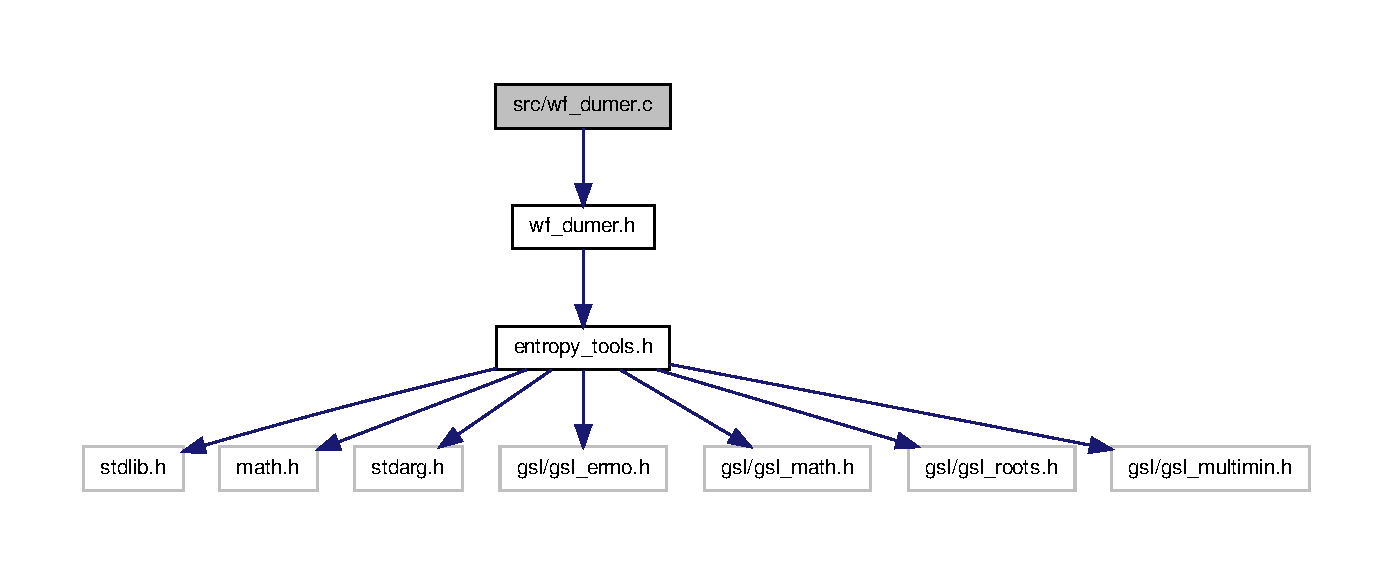
\includegraphics[width=350pt]{wf__dumer_8c__incl}
\end{center}
\end{figure}

\subsection*{\-Functions}
\begin{DoxyCompactItemize}
\item 
double \hyperlink{wf__dumer_8c_a5244b19be3abd3f78ed6cca7ecd7a01e}{wf\-\_\-\-Dumer} (const gsl\-\_\-vector $\ast$v, void $\ast$params)
\item 
double \hyperlink{wf__dumer_8c_a479daa36a2e80f4a1432e4d4b027f8a3}{\-Optimal\-\_\-wf\-\_\-\-Dumer} (\hyperlink{structwf__params}{wf\-\_\-params} $\ast$params)
\end{DoxyCompactItemize}

\subsection{\-Detailed \-Description}
\-Implementation of \hyperlink{wf__dumer_8h}{include/wf\-\_\-dumer.\-h}. 

\-Definition in file \hyperlink{wf__dumer_8c}{wf\-\_\-dumer.\-c}.

\subsection{\-Function \-Documentation}

\hypertarget{wf__dumer_8c_a5244b19be3abd3f78ed6cca7ecd7a01e}{\index{wf\-\_\-dumer.\-c@{wf\-\_\-dumer.\-c}!wf\-\_\-\-Dumer@{wf\-\_\-\-Dumer}}
\index{wf\-\_\-\-Dumer@{wf\-\_\-\-Dumer}!wf_dumer.c@{wf\-\_\-dumer.\-c}}
\subsubsection[{wf\-\_\-\-Dumer}]{\setlength{\rightskip}{0pt plus 5cm}double {\bf wf\-\_\-\-Dumer} (
\begin{DoxyParamCaption}
\item[{const gsl\-\_\-vector $\ast$}]{v, }
\item[{void $\ast$}]{params}
\end{DoxyParamCaption}
)}}\label{wf__dumer_8c_a5244b19be3abd3f78ed6cca7ecd7a01e}

Work Factor of Dumer's algorithm. Parameters l and p in v and k, w, N in params. 

\-Implementation at line 29 of file wf\-\_\-dumer.\-c.

\hypertarget{wf__dumer_8c_a479daa36a2e80f4a1432e4d4b027f8a3}{\index{wf\-\_\-dumer.\-c@{wf\-\_\-dumer.\-c}!\-Optimal\-\_\-wf\-\_\-\-Dumer@{\-Optimal\-\_\-wf\-\_\-\-Dumer}}
\index{\-Optimal\-\_\-wf\-\_\-\-Dumer@{\-Optimal\-\_\-wf\-\_\-\-Dumer}!wf_dumer.c@{wf\-\_\-dumer.\-c}}
\subsubsection[{\-Optimal\-\_\-wf\-\_\-\-Dumer}]{\setlength{\rightskip}{0pt plus 5cm}double {\bf \-Optimal\-\_\-wf\-\_\-\-Dumer} (
\begin{DoxyParamCaption}
\item[{{\bf wf\-\_\-params} $\ast$}]{params}
\end{DoxyParamCaption}
)}}\label{wf__dumer_8c_a479daa36a2e80f4a1432e4d4b027f8a3}

Optimal Work Factor of Dumer's algorithm. Parameters k, w, N in params. It saves Optimal Parameters l and p in params. 

\-Implementation at line 53 of file wf\-\_\-dumer.\-c.
\hypertarget{wf__mmt_8c}{\section{src/wf\-\_\-mmt.c \-File \-Reference}
\label{wf__mmt_8c}\index{src/wf\-\_\-mmt.\-c@{src/wf\-\_\-mmt.\-c}}
}

\subsection*{Dependencies}
{\ttfamily \#include $<$wf\-\_\-mmt.\-h$>$}\*

\-Include dependency graph for wf\-\_\-mmt.\-c\-:\nopagebreak
\begin{figure}[H]
\begin{center}
\leavevmode
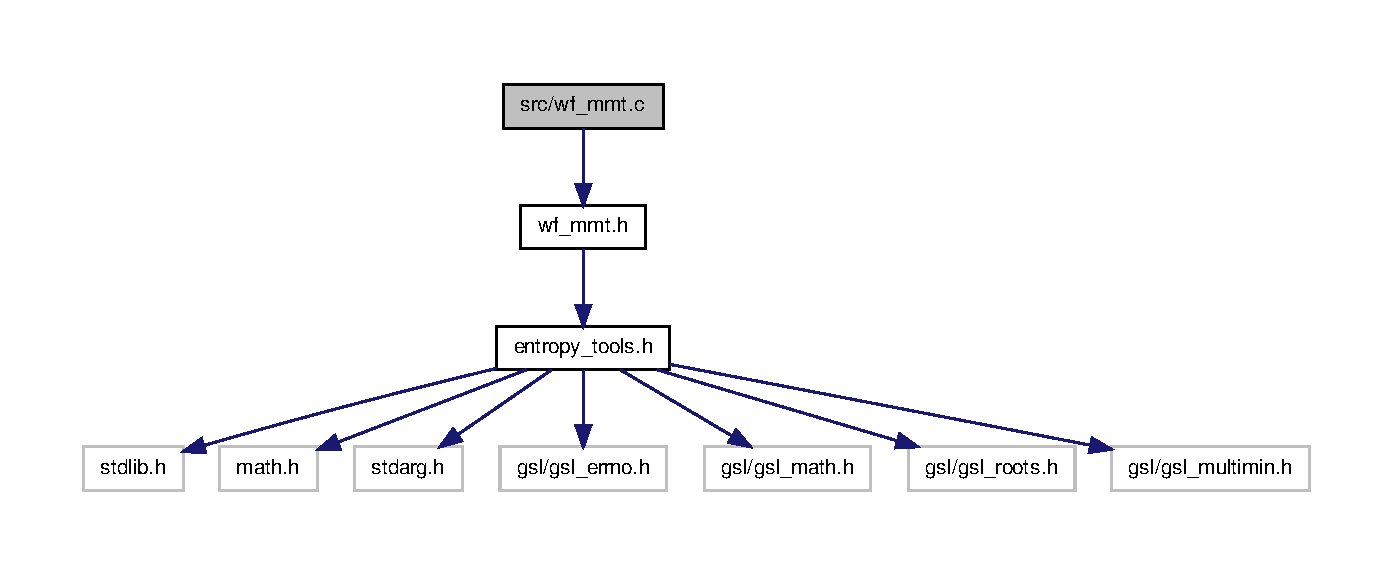
\includegraphics[width=350pt]{wf__mmt_8c__incl}
\end{center}
\end{figure}


\subsection*{\-Functions}
\begin{DoxyCompactItemize}
\item 
double \hyperlink{wf__mmt_8c_afaaf2eaa35dcf780ab4405c3f6ce8707}{wf\-\_\-\-M\-M\-T} (const gsl\-\_\-vector $\ast$v, void $\ast$params)
\item 
double \hyperlink{wf__mmt_8c_a3d6e7472113ea6b9f6e05dd8800918e6}{\-Optimal\-\_\-wf\-\_\-\-M\-M\-T} (\hyperlink{structwf__params}{wf\-\_\-params} $\ast$params)
\end{DoxyCompactItemize}


\subsection{\-Detailed \-Description}
\-Implementation of \hyperlink{wf__mmt_8h}{include/wf\-\_\-mmt.\-h}. 
\-Definition in file \hyperlink{wf__mmt_8c}{wf\-\_\-mmt.\-c}.


\subsection{\-Function \-Documentation}


\hypertarget{wf__mmt_8c_afaaf2eaa35dcf780ab4405c3f6ce8707}{\index{wf\-\_\-mmt.\-c@{wf\-\_\-mmt.\-c}!wf\-\_\-\-M\-M\-T@{wf\-\_\-\-M\-M\-T}}
\index{wf\-\_\-\-M\-M\-T@{wf\-\_\-\-M\-M\-T}!wf_mmt.c@{wf\-\_\-mmt.\-c}}
\subsubsection[{wf\-\_\-\-M\-M\-T}]{\setlength{\rightskip}{0pt plus 5cm}double {\bf wf\-\_\-\-M\-M\-T} (
\begin{DoxyParamCaption}
\item[{const gsl\-\_\-vector $\ast$}]{v, }
\item[{void $\ast$}]{params}
\end{DoxyParamCaption}
)}}\label{wf__mmt_8c_afaaf2eaa35dcf780ab4405c3f6ce8707}


\-Work \-Factor of \-M\-M\-T's algorithm. Parameters l and p in gsl\-\_\-vector v and k, w, \-N in params. 

\-Implementation at line 29 of file wf\-\_\-mmt.\-c.


\hypertarget{wf__mmt_8c_a3d6e7472113ea6b9f6e05dd8800918e6}{\index{wf\-\_\-mmt.\-c@{wf\-\_\-mmt.\-c}!\-Optimal\-\_\-wf\-\_\-\-M\-M\-T@{\-Optimal\-\_\-wf\-\_\-\-M\-M\-T}}
\index{\-Optimal\-\_\-wf\-\_\-\-M\-M\-T@{\-Optimal\-\_\-wf\-\_\-\-M\-M\-T}!wf_mmt.c@{wf\-\_\-mmt.\-c}}
\subsubsection[{\-Optimal\-\_\-wf\-\_\-\-M\-M\-T}]{\setlength{\rightskip}{0pt plus 5cm}double {\bf \-Optimal\-\_\-wf\-\_\-\-M\-M\-T} (
\begin{DoxyParamCaption}
\item[{{\bf wf\-\_\-params} $\ast$}]{params}
\end{DoxyParamCaption}
)}}\label{wf__mmt_8c_a3d6e7472113ea6b9f6e05dd8800918e6}


\-Optimal \-Work \-Factor of \-M\-M\-T's algorithm. Parameters k, w, \-N in params. \-It saves \-Optimal \-Parameters l and p in params. 

\-Implementation at line 52 of file wf\-\_\-mmt.\-c.


\hypertarget{wf__nn_8c}{\section{src/wf\-\_\-nn.c \-File \-Reference}
\label{wf__nn_8c}\index{src/wf\-\_\-nn.\-c@{src/wf\-\_\-nn.\-c}}
}


\-Implementation of \hyperlink{wf__nn_8h}{include/wf\-\_\-nn.\-h}.  

\subsection*{Dependencies}

{\ttfamily \#include $<$wf\-\_\-nn.\-h$>$}\*\\

\-Include dependency graph for wf\-\_\-nn.\-c\-:\nopagebreak
\begin{figure}[H]
\begin{center}
\leavevmode
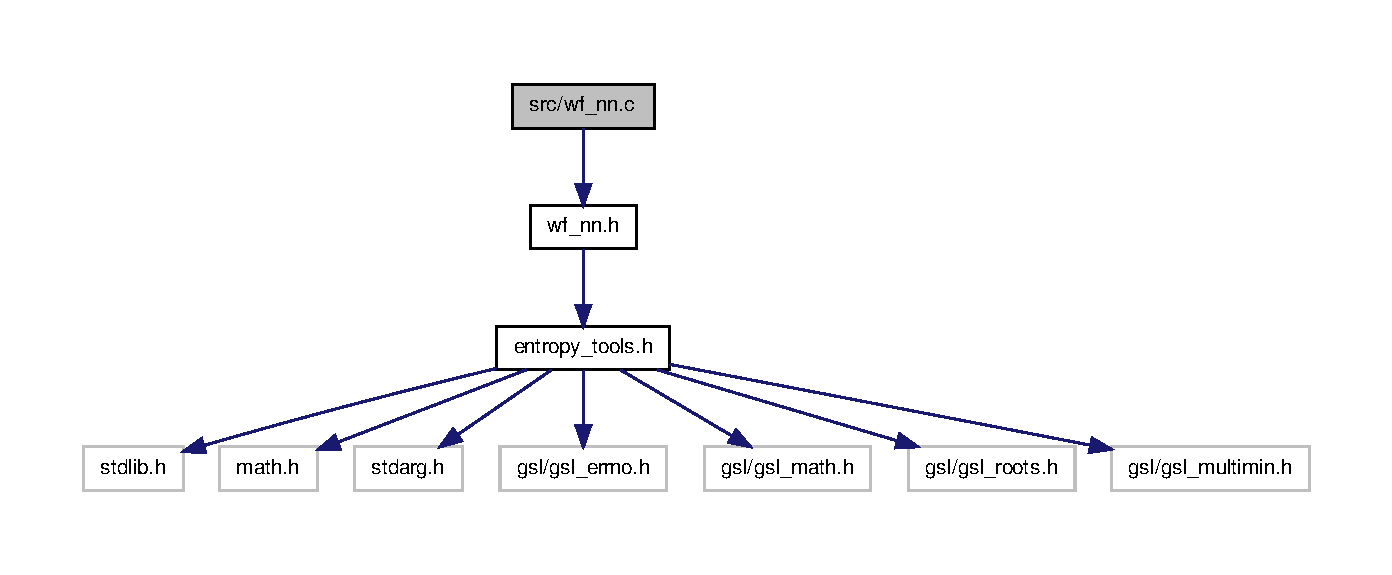
\includegraphics[width=350pt]{wf__nn_8c__incl}
\end{center}
\end{figure}

\subsection*{\-Functions}
\begin{DoxyCompactItemize}
\item 
double \hyperlink{wf__nn_8c_a8dfefc665bca9dae6c43d725c23e6744}{wf\-\_\-\-N\-N} (double p2, void $\ast$paramslpp1)
\item 
double \hyperlink{wf__nn_8c_ad2f6d42b4446e77ad8c5d132f7535383}{\-Optimal\-\_\-wf\-\_\-\-N\-N\-\_\-p} (const gsl\-\_\-vector $\ast$v, void $\ast$params)
\item 
double \hyperlink{wf__nn_8c_aabe262ad8c85dbe0c434cba3463bd955}{\-Optimal\-\_\-wf\-\_\-\-N\-N} (\hyperlink{structwf__params}{wf\-\_\-params} $\ast$params)
\end{DoxyCompactItemize}


\subsection{\-Detailed \-Description}
\-Implementation of \hyperlink{wf__nn_8h}{include/wf\-\_\-nn.\-h}. 

\-Definition in file \hyperlink{wf__nn_8c}{wf\-\_\-nn.\-c}.



\subsection{\-Function \-Documentation}

\hypertarget{wf__nn_8c_a8dfefc665bca9dae6c43d725c23e6744}{\index{wf\-\_\-nn.\-c@{wf\-\_\-nn.\-c}!wf\-\_\-\-N\-N@{wf\-\_\-\-N\-N}}
\index{wf\-\_\-\-N\-N@{wf\-\_\-\-N\-N}!wf_nn.c@{wf\-\_\-nn.\-c}}
\subsubsection[{wf\-\_\-\-N\-N}]{\setlength{\rightskip}{0pt plus 5cm}double {\bf wf\-\_\-\-N\-N} (
\begin{DoxyParamCaption}
\item[{double}]{p2, }
\item[{void $\ast$}]{paramslpp1}
\end{DoxyParamCaption}
)}}\label{wf__nn_8c_a8dfefc665bca9dae6c43d725c23e6744}


\-Work \-Factor of \-Nearest \-Neighbord's algorithm. Parameters k, w, \-N, l ,p, p1 in paramslpp1.

\-Implementation at line 29 of file wf\-\_\-nn.\-c.

\hypertarget{wf__nn_8c_ad2f6d42b4446e77ad8c5d132f7535383}{\index{wf\-\_\-nn.\-c@{wf\-\_\-nn.\-c}!\-Optimal\-\_\-wf\-\_\-\-N\-N\-\_\-p@{\-Optimal\-\_\-wf\-\_\-\-N\-N\-\_\-p}}
\index{\-Optimal\-\_\-wf\-\_\-\-N\-N\-\_\-p@{\-Optimal\-\_\-wf\-\_\-\-N\-N\-\_\-p}!wf_nn.c@{wf\-\_\-nn.\-c}}
\subsubsection[{\-Optimal\-\_\-wf\-\_\-\-N\-N\-\_\-p}]{\setlength{\rightskip}{0pt plus 5cm}double {\bf \-Optimal\-\_\-wf\-\_\-\-N\-N\-\_\-p} (
\begin{DoxyParamCaption}
\item[{const gsl\-\_\-vector $\ast$}]{v, }
\item[{void $\ast$}]{params}
\end{DoxyParamCaption}
)}}\label{wf__nn_8c_ad2f6d42b4446e77ad8c5d132f7535383}


\-Optimal \-Work \-Factor of \-Nearest \-Neighbord's algorithm for l, p fixed. Parameters l and p in v and k, w, \-N in params. \-It saves \-Optimal \-Parameters p2 in paramslp ( p1 is chosen from l and p).

\-Implementation at line 62 of file wf\-\_\-nn.\-c.



\hypertarget{wf__nn_8c_aabe262ad8c85dbe0c434cba3463bd955}{\index{wf\-\_\-nn.\-c@{wf\-\_\-nn.\-c}!\-Optimal\-\_\-wf\-\_\-\-N\-N@{\-Optimal\-\_\-wf\-\_\-\-N\-N}}
\index{\-Optimal\-\_\-wf\-\_\-\-N\-N@{\-Optimal\-\_\-wf\-\_\-\-N\-N}!wf_nn.c@{wf\-\_\-nn.\-c}}
\subsubsection[{\-Optimal\-\_\-wf\-\_\-\-N\-N}]{\setlength{\rightskip}{0pt plus 5cm}double {\bf \-Optimal\-\_\-wf\-\_\-\-N\-N} (
\begin{DoxyParamCaption}
\item[{{\bf wf\-\_\-params} $\ast$}]{params}
\end{DoxyParamCaption}
)}}\label{wf__nn_8c_aabe262ad8c85dbe0c434cba3463bd955}


\-Optimal \-Work \-Factor of \-Nearest \-Neighbord's algorithm. Parameters k, w, \-N in params. \-It saves \-Optimal \-Parameters l, p, p1 and p2 in params. 

\-Implementation at line 122 of file wf\-\_\-nn.\-c.
\hypertarget{wf__prange_8c}{\section{src/wf\-\_\-prange.c \-File \-Reference}
\label{wf__prange_8c}\index{src/wf\-\_\-prange.\-c@{src/wf\-\_\-prange.\-c}}
}


\-Implementation of \hyperlink{wf__prange_8h}{include/wf\-\_\-prange.\-h}.  

\subsection*{Dependencies}
{\ttfamily \#include $<$wf\-\_\-prange.\-h$>$}\*

\-Include dependency graph for wf\-\_\-prange.\-c\-:\nopagebreak
\begin{figure}[H]
\begin{center}
\leavevmode
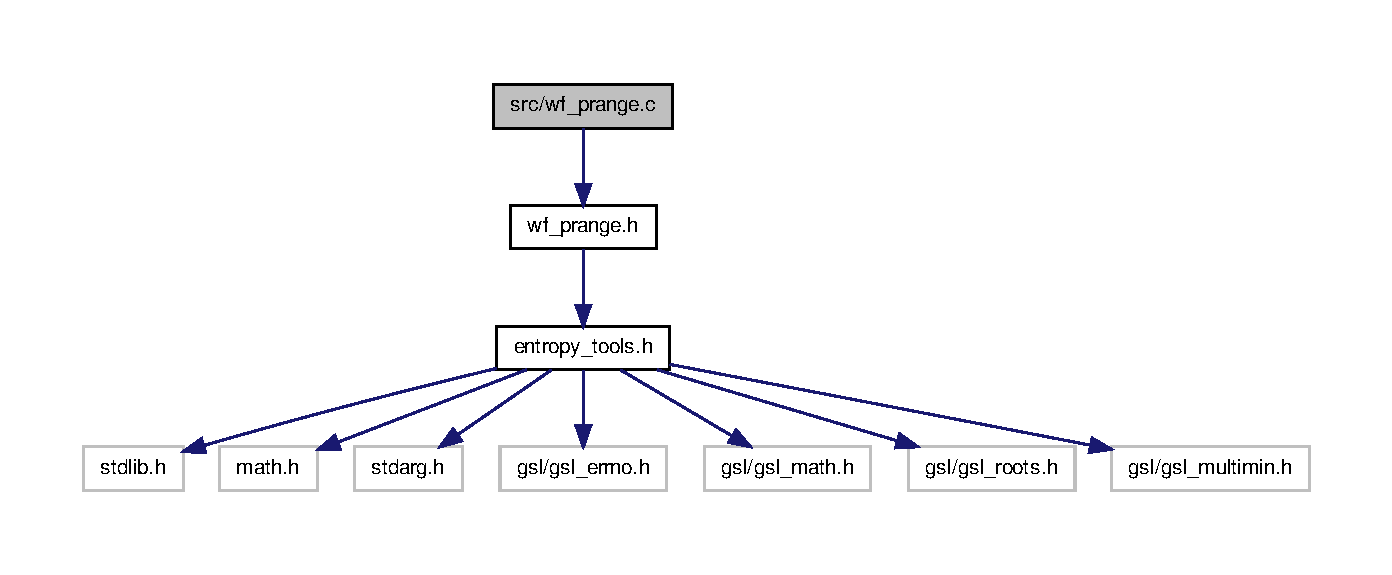
\includegraphics[width=350pt]{wf__prange_8c__incl}
\end{center}
\end{figure}


\subsection*{\-Functions}
\begin{DoxyCompactItemize}
\item 
double \hyperlink{wf__prange_8c_aaab4db55369e553a26cfe4de8fb9ecb8}{wf\-\_\-\-Prange} (\hyperlink{structwf__params}{wf\-\_\-params} $\ast$params)
\end{DoxyCompactItemize}


\subsection{\-Detailed \-Description}
\-Implementation of \hyperlink{wf__prange_8h}{include/wf\-\_\-prange.\-h}. 

\-Definition in file \hyperlink{wf__prange_8c}{wf\-\_\-prange.\-c}.



\subsection{\-Function \-Documentation}
\hypertarget{wf__prange_8c_aaab4db55369e553a26cfe4de8fb9ecb8}{\index{wf\-\_\-prange.\-c@{wf\-\_\-prange.\-c}!wf\-\_\-\-Prange@{wf\-\_\-\-Prange}}
\index{wf\-\_\-\-Prange@{wf\-\_\-\-Prange}!wf_prange.c@{wf\-\_\-prange.\-c}}
\subsubsection[{wf\-\_\-\-Prange}]{\setlength{\rightskip}{0pt plus 5cm}double {\bf wf\-\_\-\-Prange} (
\begin{DoxyParamCaption}
\item[{{\bf wf\-\_\-params} $\ast$}]{params}
\end{DoxyParamCaption}
)}}\label{wf__prange_8c_aaab4db55369e553a26cfe4de8fb9ecb8}

Work Factor of Prange's algorithm. 

\-Implementation at line 29 of file wf\-\_\-prange.\-c.


\hypertarget{wf__stern_8c}{\section{src/wf\-\_\-stern.c \-File \-Reference}
\label{wf__stern_8c}\index{src/wf\-\_\-stern.\-c@{src/wf\-\_\-stern.\-c}}
}


\-Implementation of \hyperlink{wf__stern_8h}{include/wf\-\_\-stern.\-h}.  

\subsection*{Dependencies}

{\ttfamily \#include $<$wf\-\_\-stern.\-h$>$}\*\\

\begin{figure}[H]
\begin{center}
\leavevmode
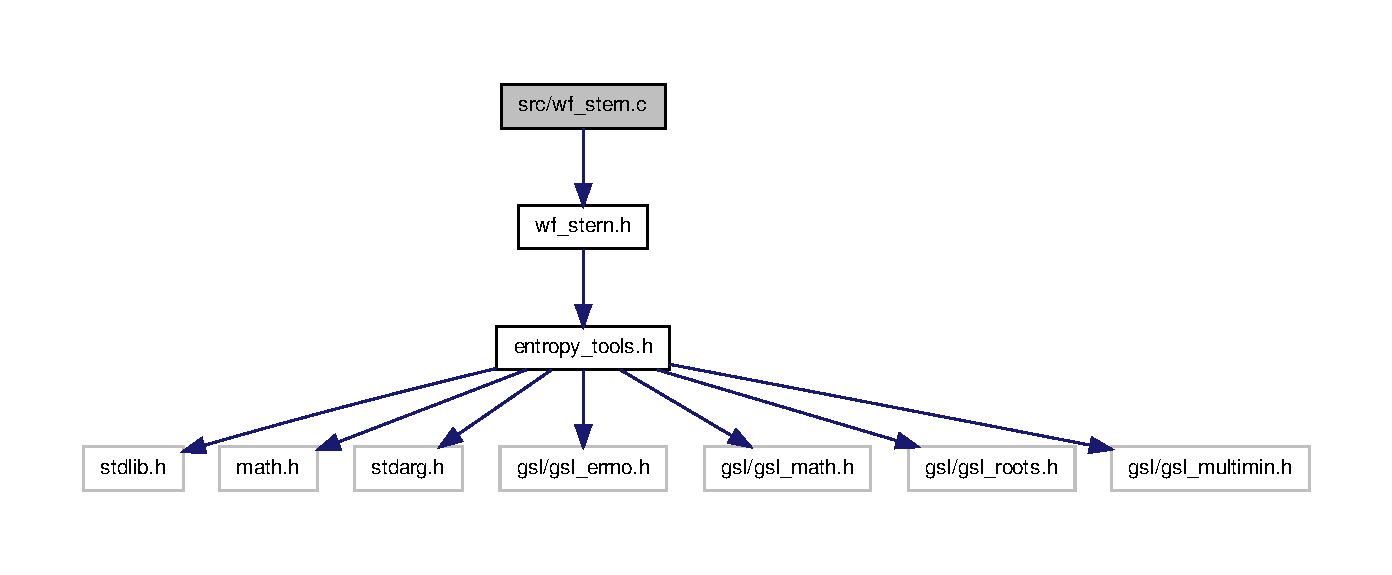
\includegraphics[width=350pt]{wf__stern_8c__incl}
\end{center}
\end{figure}
\subsection*{\-Functions}
\begin{DoxyCompactItemize}
\item 
double \hyperlink{wf__stern_8c_a79ee922bb25d99869ec7f0fb94a109cc}{wf\-\_\-\-Stern} (const gsl\-\_\-vector $\ast$v, void $\ast$params)
\item 
double \hyperlink{wf__stern_8c_ad0f06aed633e1453adc6f85a5d1d35b2}{\-Optimal\-\_\-wf\-\_\-\-Stern} (\hyperlink{structwf__params}{wf\-\_\-params} $\ast$params)
\end{DoxyCompactItemize}


\subsection{\-Detailed \-Description}
\-Implementation of \hyperlink{wf__stern_8h}{include/wf\-\_\-stern.\-h}.

\-Definition in file \hyperlink{wf__stern_8c}{wf\-\_\-stern.\-c}.

\subsection{\-Function \-Documentation}
\hypertarget{wf__stern_8c_a79ee922bb25d99869ec7f0fb94a109cc}{\index{wf\-\_\-stern.\-c@{wf\-\_\-stern.\-c}!wf\-\_\-\-Stern@{wf\-\_\-\-Stern}}
\index{wf\-\_\-\-Stern@{wf\-\_\-\-Stern}!wf_stern.c@{wf\-\_\-stern.\-c}}
\subsubsection[{wf\-\_\-\-Stern}]{\setlength{\rightskip}{0pt plus 5cm}double {\bf wf\-\_\-\-Stern} (
\begin{DoxyParamCaption}
\item[{const gsl\-\_\-vector $\ast$}]{v, }
\item[{void $\ast$}]{params}
\end{DoxyParamCaption}
)}}\label{wf__stern_8c_a79ee922bb25d99869ec7f0fb94a109cc}

Work Factor of Stern's algorithm. Parameters l and p in v and k, w, N in params. 

\-Implementation at line 29 of file wf\-\_\-stern.\-c.

\hypertarget{wf__stern_8c_ad0f06aed633e1453adc6f85a5d1d35b2}{\index{wf\-\_\-stern.\-c@{wf\-\_\-stern.\-c}!\-Optimal\-\_\-wf\-\_\-\-Stern@{\-Optimal\-\_\-wf\-\_\-\-Stern}}
\index{\-Optimal\-\_\-wf\-\_\-\-Stern@{\-Optimal\-\_\-wf\-\_\-\-Stern}!wf_stern.c@{wf\-\_\-stern.\-c}}
\subsubsection[{\-Optimal\-\_\-wf\-\_\-\-Stern}]{\setlength{\rightskip}{0pt plus 5cm}double {\bf \-Optimal\-\_\-wf\-\_\-\-Stern} (
\begin{DoxyParamCaption}
\item[{{\bf wf\-\_\-params} $\ast$}]{params}
\end{DoxyParamCaption}
)}}\label{wf__stern_8c_ad0f06aed633e1453adc6f85a5d1d35b2}

\-Optimal \-Work \-Factor of \-Stern's algorithm. Parameters k, w, \-N in params. \-It saves \-Optimal \-Parameters l and p in params. 

\-Implementation at line 53 of file wf\-\_\-stern.\-c.
\printindex
\end{document}
